\section{Experimental Results}
\subsection{Example Regression Problem}
This problem serves as a quick example to demonstrate many of the phenomena described in previous sections. We trained two networks to learn the cosine function, with one input and one output. This is a task which requires no more than 11 sigmoid neurons to solve entirely, and in this case we don't care about overfitting because the cosine function has a precise definition. Furthermore, the cosine function is a good toy example because it is a smooth continuous function and, as demonstrated by \cite{nielsen2015neural}, if we were to tinker directly with the weights and bias parameters of the network, we could allocate individual units within the network to be responsible for constrained ranges of inputs, similar to a basis spline function with many control points. This would distribute the learned function approximation evenly across all hidden units, and thus we have presented the network with a problem in which it could productively use as many hidden units as we give it. In this case, a pruning algorithm would observe a fairly consistent increase in error after the removal of each successive unit. In practice however, regardless of the number of experimental trials, this is not what happens. The network will always use 10-11 hidden units and leave the rest to cancel each other's influence.

\begin{figure}[!ht]
\centering
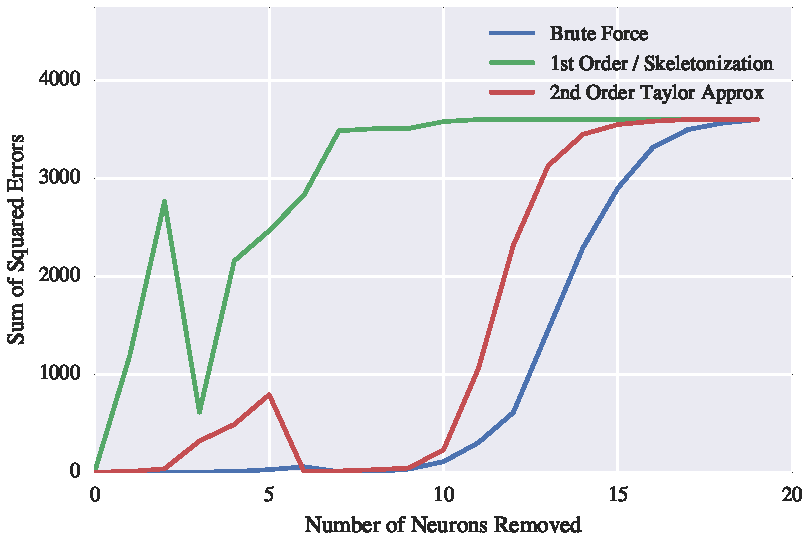
\includegraphics[width=0.49\linewidth]{cos-small.pdf}
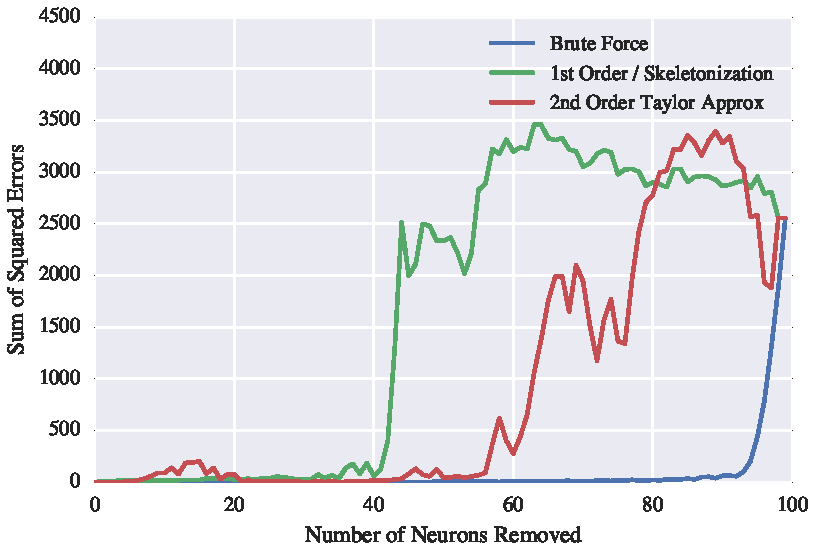
\includegraphics[width=0.49\linewidth]{cos-big.pdf}
\caption{Degradation in squared error after pruning a two-layer network trained to compute the cosine function (\textbf{Left Network:} 2 layers, 10 neurons each, 1 output, logistic sigmoid activation, starting test accuracy: 0.9999993, \textbf{Right Network:} 2 layers, 50 neurons each, 1 output, logistic sigmoid activation, starting test accuracy: 0.9999996)}
\label{fig:cosine-double-layer}
\end{figure}

Figure \ref{fig:cosine-double-layer} shows two graphs. Both graphs demonstrate the use of the iterative re-ranking algorithm and the comparative performance of the brute-force pruning method (in blue), the first order method (in green), and the second order method (in red). The graph on the left shows the performance of these algorithms starting from a network with two layers of 10 neurons (20 total), and the graph on the right shows a network with two layers of 50 neurons (100 total). 

In the left graph, we see that the brute-force method shows a graceful degradation, and the error only begins to rise sharply after 50\% of the total neurons have been removed. The error is basically constant up to that point. In the first and second order methods, we see evidence of poor decision making in the sense that both made mistakes early on, which disrupted the output function approximation. The first order method made a large error early on, though we see after a few more neurons were removed this error was corrected somewhat (though it only got worse from there). This is direct evidence of the lack of fault tolerance in a trained neural network. This phenomenon is even more starkly demonstrated in the second order method. After making a few poor neuron removal decisions in a row, the error signal rose sharply, and then went back to zero after the 6th neuron was removed. This is due to the fact that the neurons it chose to remove were trained to cancel each others' influence within a localized part of the network. After the entire group was eliminated, the approximation returned to normal. This can only happen if the output function approximation is not evenly distributed over the hidden units in a trained network. 

This phenomenon is even more starkly demonstrated in the graph on the right. Here we see the first order method got ``lucky'' in the beginning and made decent decisions up to about the 40th removed neuron. The second order method had a small error in the beginning which it recovered from gracefully and proceeded to pass the 50 neuron point before finally beginning to unravel. The brute force method, in sharp contrast, shows little to no increase in error at all until 90\% of the neurons in the network have been obliterated. Clearly first and second order methods have some value in that they do not make completely arbitrary choices, but the brute force method is far better at this task. 

This also demonstrates the sharp dualism in neuron roles within a trained network. These networks were trained to near-perfect precision and each pruning method was applied \textit{without} any re-training of any kind. Clearly, in the case of the brute force or oracle method, up to 90\% of the network can be completely extirpated before the output approximation even begins to show any signs of degradation. This would be impossible if the learning representation were evenly or equitably distributed. Note, for example, that the degradation point in both cases is approximately the same. This example is not a real-world application of course, but it brings into very clear focus the kind of phenomena we will discuss in the following sections. 

\subsection{Results on MNIST Dataset}
For all the results presented in this section, the MNIST database of Handwritten Digits by \cite{lecun-mnisthandwrittendigit-2010} was used. It is worth noting that due to the time taken by the brute force algorithm we rather used a 5000 image subset of the MNIST database in which we have normalized the pixel values between 0 and 1.0, and compressed the image sizes to 20x20 images rather than 28x28, so the starting test accuracy reported here appears higher than those reported by LeCun et al. We do not believe that this affects the interpretation of the presented results because the basic learning problem does not change with a larger dataset or input dimension.

\subsection{Pruning a 1-Layer Network}
The network architecture in this case consisted of 1 layer, 100 neurons, 10 outputs, logistic sigmoid activations, and a starting test accuracy of 0.998.

\subsubsection{Single Overall Ranking Algorithm}
We first present the results for a single-layer neural network in Figure \ref{fig:mnist-single-ranking-single-layer}, using the Single Overall algorithm (Algorithm \ref{algo1}) as proposed in Section \ref{sec2}. (We again note that this algorithm is intentionally naive and is used for comparison only. Its performance should be expected to be poor.) After training, each neuron is assigned its permanent ranking based on the three criteria discussed previously: A brute force ``ground truth'' ranking, and two approximations of this ranking using first and second order Taylor estimations of the change in network output error resulting from the removal of each neuron. 

\begin{figure}[!ht]
\centering
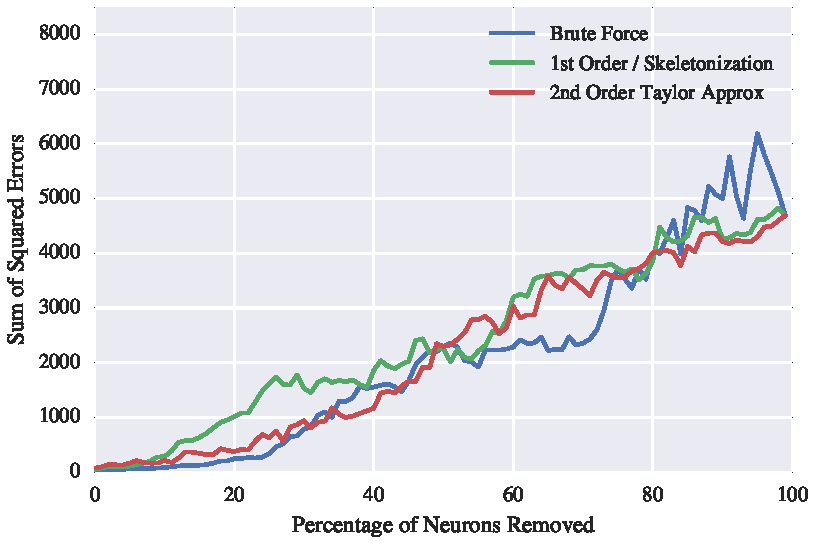
\includegraphics[width=0.49\linewidth]{mnist-acc99-single-pass-method.pdf}
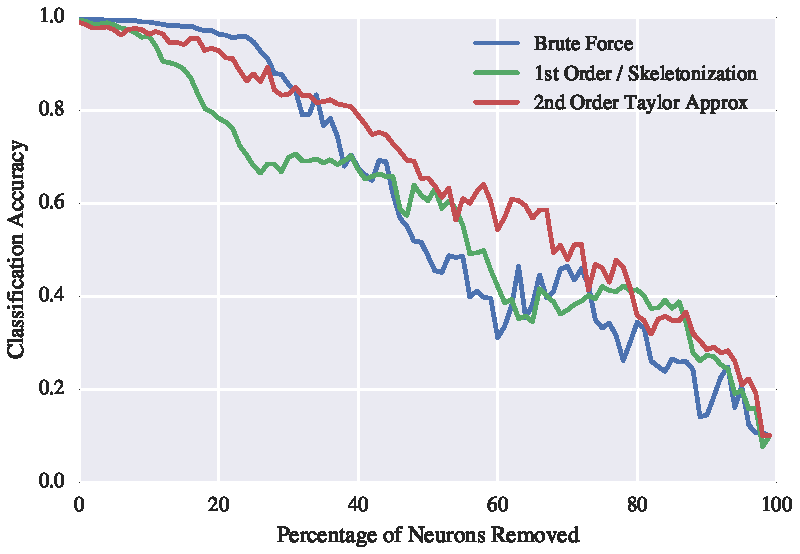
\includegraphics[width=0.49\linewidth]{mnist-acc99-single-pass-accuracy.pdf}
\caption{Degradation in squared error (left) and classification accuracy (right) after pruning a single-layer network using The Single Overall Ranking algorithm (\textbf{Network:} 1 layer, 100 neurons, 10 outputs, logistic sigmoid activation, starting test accuracy: 0.998)}
\label{fig:mnist-single-ranking-single-layer}
\end{figure}

An interesting observation here is that with only a single layer, no criteria for ranking the neurons in the network (brute force or the two Taylor Series variants) using Algorithm \ref{algo1} emerges superior, indicating that the 1st and 2nd order Taylor Series methods are actually reasonable approximations of the brute force method under certain conditions. Of course, this method is still quite bad in terms of the rate of degradation of the classification accuracy and in practice we would likely follow Algorithm \ref{algo2} which is takes into account \cite{mozer1989skeletonization}'s observations stated in the Related Work section. The purpose of the present investigation, however, is to demonstrate how much of a trained network can be theoretically removed without altering the network's learned parameters in any way.

\subsubsection{Iterative Re-Ranking Algorithm}
\begin{figure}[!ht]
\centering
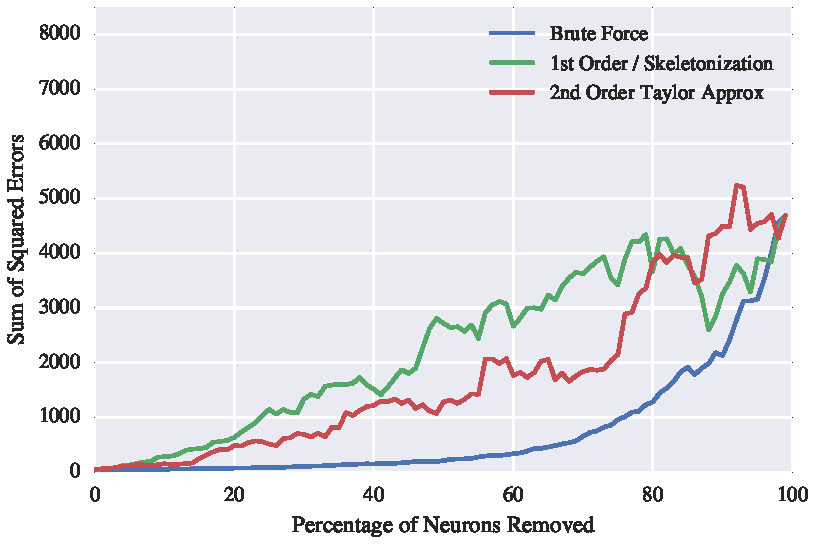
\includegraphics[width=0.49\linewidth]{mnist-acc99-iterative-rerank-method.pdf}
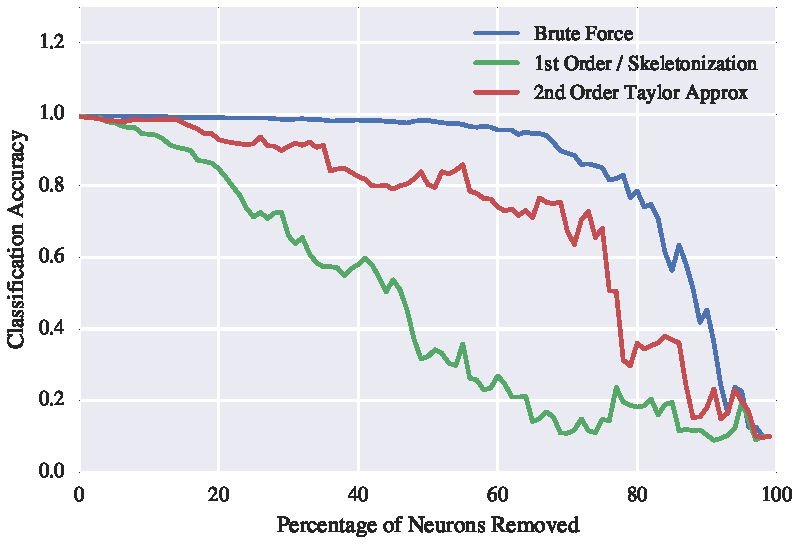
\includegraphics[width=0.49\linewidth]{mnist-acc99-iterative-rerank-accuracy.pdf}
\caption{Degradation in squared error (left) and classification accuracy (right) after pruning a single-layer network the iterative re-ranking algorithm (\textbf{Network:} 1 layer, 100 neurons, 10 outputs, logistic sigmoid activation, starting test accuracy: 0.998)}
\label{fig:mnist-re-ranking-single-layer}
\end{figure}

In Figure \ref{fig:mnist-re-ranking-single-layer} we present our results using Algorithm \ref{algo2} (The iterative re-ranking Algorithm) in which all remaining neurons are re-ranked after each successive neuron is switched off. We compute the same brute force rankings and Taylor series approximations of error deltas over the remaining active neurons in the network after each pruning decision. This is intended to account for the effects of cancelling interactions between neurons. 

There are 2 key observations here. Using the brute force ranking criteria, almost 60\% of the neurons in the network can be pruned away without any major loss in performance. The other noteworthy observation here is that the 2nd order Taylor Series approximation of the error performs consistently better than its 1st order version, in most situations, though Figure \ref{fig:mnist-test-single-digit-2} is a poignant counter-example. 

%tl;dr: 1 layer is grrrreat for brute force! Clearly 2nd order method is consistently better than 1st order method. 

%tl;dr: Brute force method is amazing here! 1 layer makes things a lot easier, and a 2nd order method can do okay as well, but can still be improved a lot. 60% of neurons doing nothing!

\subsubsection{Visualization of Error Surface \& Pruning Decisions}

As explained in Section \ref{sec2}, these graphs are a visualization of the error surface of the network output with respect to the neurons chosen for removal using each of the 3 ranking criteria, represented in intervals of 10 neurons. In each graph, the error surface of the network output is displayed in log space (left) and in real space (right) with respect to each candidate neuron chosen for removal. We create these plots during the pruning exercise by picking a neuron to switch off, and then multiplying its output by a scalar gain value $\alpha$ which is adjusted from 0.0 to 10.0 with a step size of 0.001. When the value of $\alpha$ is 1.0, this represents the unperturbed neuron output learned during training. Between 0.0 and 1.0, we are graphing the literal effect of turning the neuron off ($\alpha = 0$), and when $\alpha > 1.0$ we are simulating a boosting of the neuron's influence in the network, i.e. inflating the value of its outgoing weight parameters. 

We graph the effect of boosting the neuron's output to demonstrate that for certain neurons in the network, even doubling, tripling, or quadrupling the scalar output of the neuron has no effect on the overall error of the network, indicating the remarkable degree to which the network has learned to ignore the value of certain parameters. In other cases, we can get a sense of the sensitivity of the network's output to the value of a given neuron when the curve rises steeply after the red 1.0 line. This indicates that the learned value of the parameters emanating from a given neuron are relatively important, and this is why we should ideally see sharper upticks in the curves for the later-removed neurons in the network, that is, when the neurons crucial to the learning representation start to be picked off. Some very interesting observations can be made in each of these graphs. 

Remember that lower is better in terms of the height of the curve and minimal (or negative) horizontal change between the vertical red line at 1.0 (neuron \textit{on}, $\alpha = 1.0$) and 0.0 (neuron \textit{off}, $\alpha = 0.0$) is indicative of a good candidate neuron to prune, i.e. there will be minimal effect on the network output when the neuron is removed. 

\subsubsection{Visualization of brute force Pruning Decisions}
\begin{figure}[!ht]
\centering
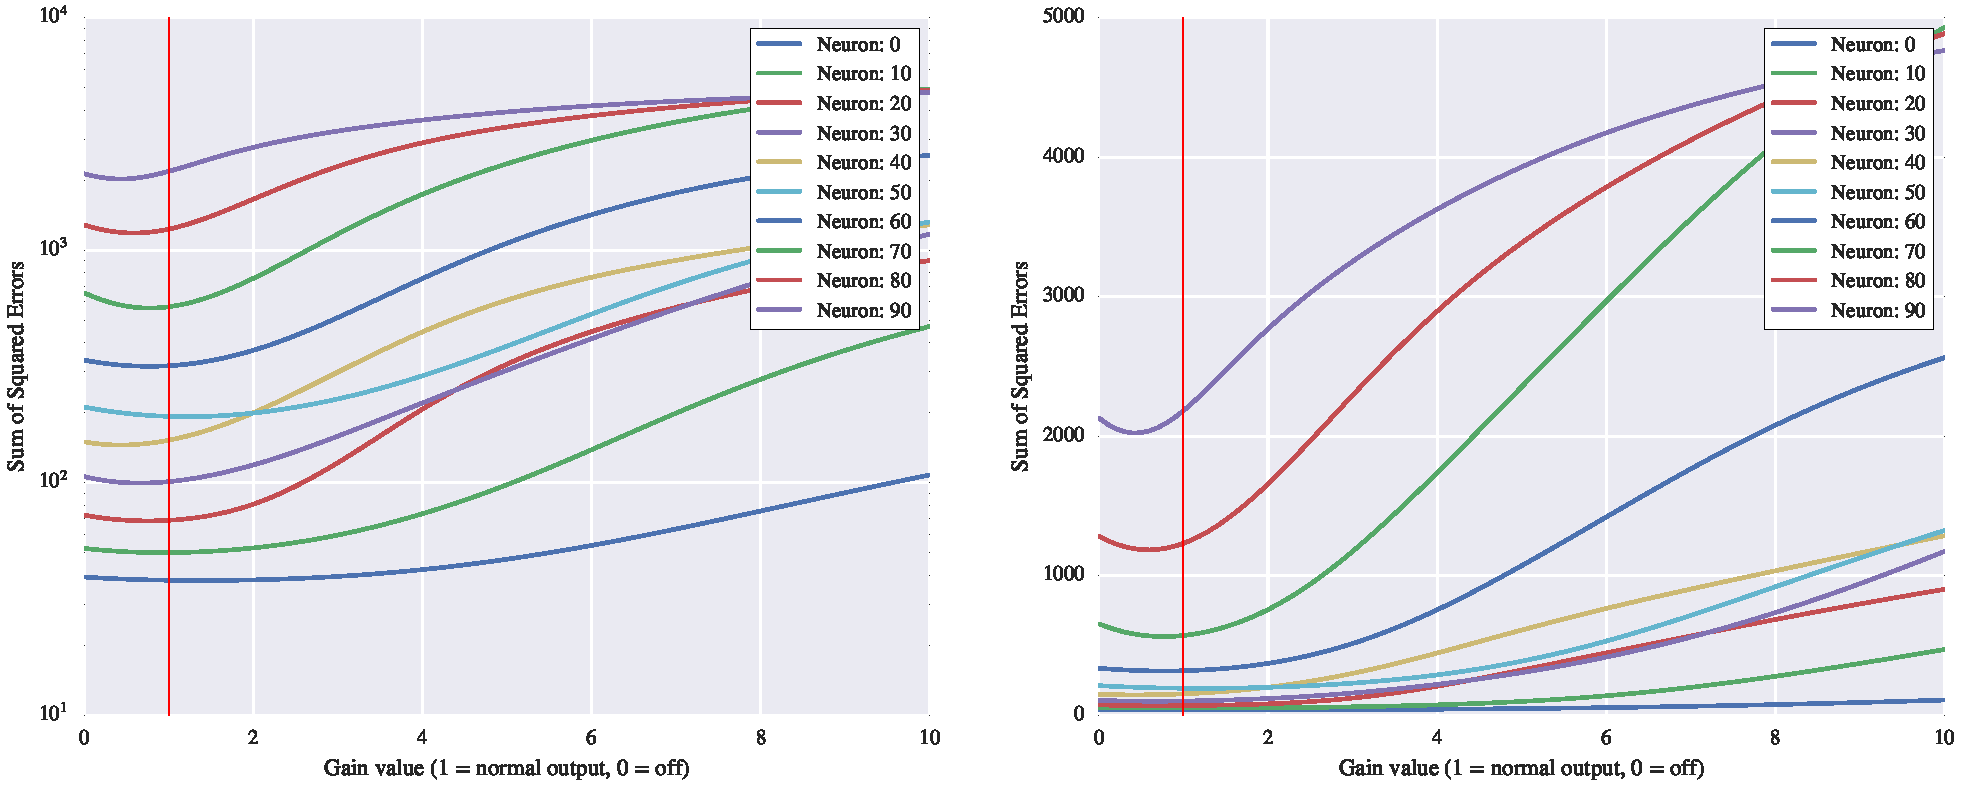
\includegraphics[width=\linewidth]{mnist-acc99-gt-gain.pdf}
\caption{Error surface of the network output in log space (left) and real space (right) with respect to each candidate neuron chosen for removal using the brute force criterion; (\textbf{Network:} 1 layer, 100 neurons, 10 outputs, logistic sigmoid activation, starting test accuracy: 0.998)}
\label{fig:mnist-single-layer-gt}
\end{figure}

In Figure \ref{fig:mnist-gt-single-layer}, we notice how low to the floor and flat most of the curves are. It's only until the 90th removed neuron that we see a higher curve with a more convex shape (clearly a more sensitive, influential piece of the network). 

\subsubsection{Visualization of 1st Order Approximation Pruning Decisions}
\begin{figure}[!ht]
\centering
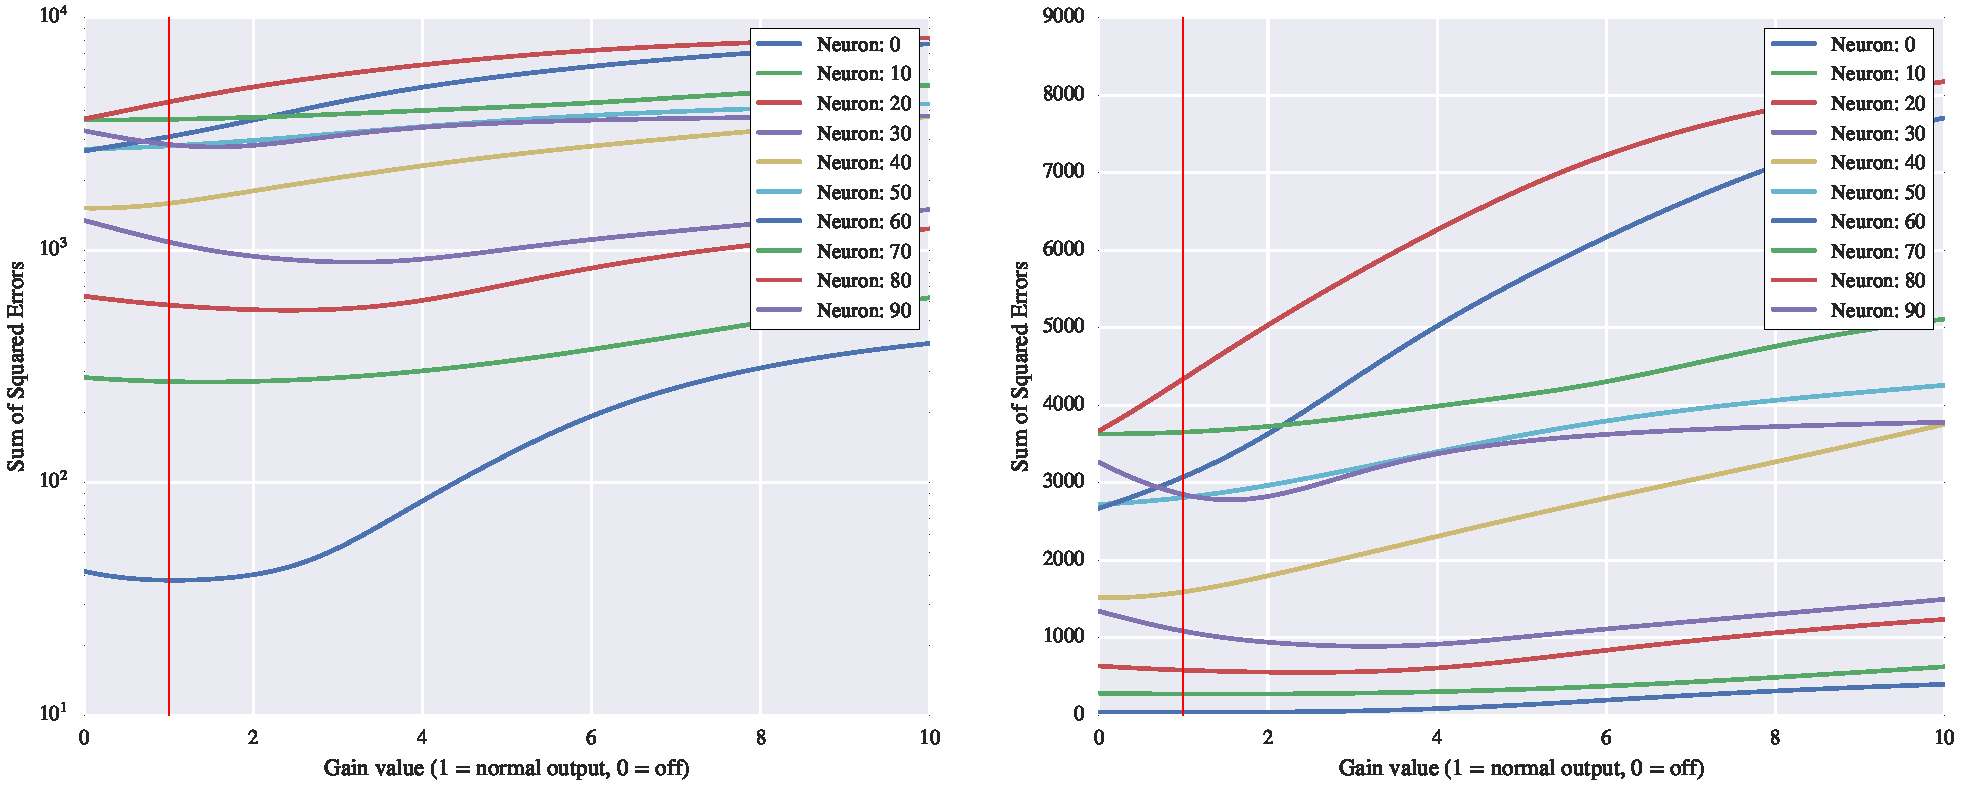
\includegraphics[width=\linewidth]{mnist-acc99-g1-gain.pdf}
\caption{Error surface of the network output in log space (left) and real space (right) with respect to each candidate neuron chosen for removal using the 1st order Taylor Series error approximation criterion; (\textbf{Network:} 1 layer, 100 neurons, 10 outputs, logistic sigmoid activation, starting test accuracy: 0.998)}
\label{fig:mnist-single-layer-g1}
\end{figure}

It can be seen in Figure \ref{fig:mnist-single-layer-g1} that most choices seem to have flat or negatively sloped curves, indicating that the first order approximation seems to be pretty good, but examining the brute force choices shows they could be better. 

\subsubsection{Visualization of 2nd Order Approximation Pruning Decisions}
\begin{figure}[!ht]
\centering
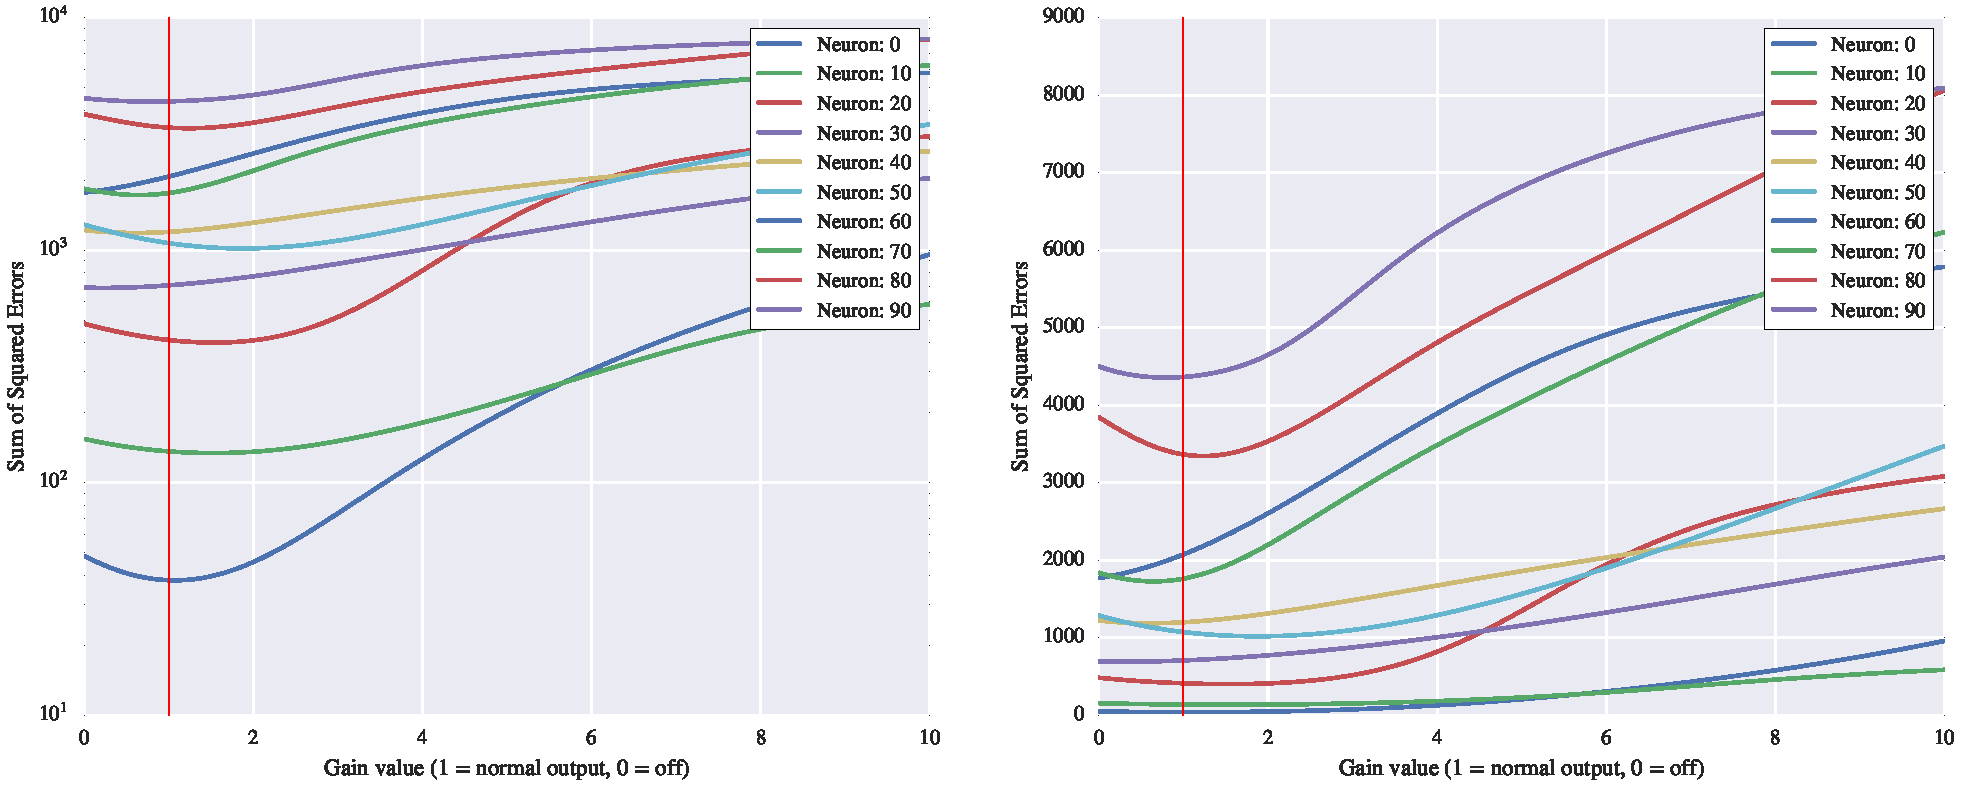
\includegraphics[width=\linewidth]{mnist-acc99-g2-gain.pdf}
\caption{Error surface of the network output in log space (left) and real space (right) with respect to each candidate neuron chosen for removal using the 2nd order Taylor Series error approximation criterion; (\textbf{Network:} 1 layer, 100 neurons, 10 outputs, logistic sigmoid activation, starting test accuracy: 0.998)}
\label{fig:mnist-single-layer-g2}
\end{figure}

The method in Figure \ref{fig:mnist-single-layer-g2} looks similar to the brute force method choices, though clearly not as good (they're more spread out). Notice the difference in convexity between the 2nd and 1st order method choices. It's clear that the first order method is fitting a line and the 2nd order method is fitting a parabola in their approximation. 

\subsection{Pruning A 2-Layer Network}
The network architecture in this case consisted of 2 layers, 50 neurons per layer, 10 outputs, logistic sigmoid activations, and a starting test accuracy of 1.000.

\subsubsection{Single Overall Ranking Algorithm}
\begin{figure}[!ht]
\centering
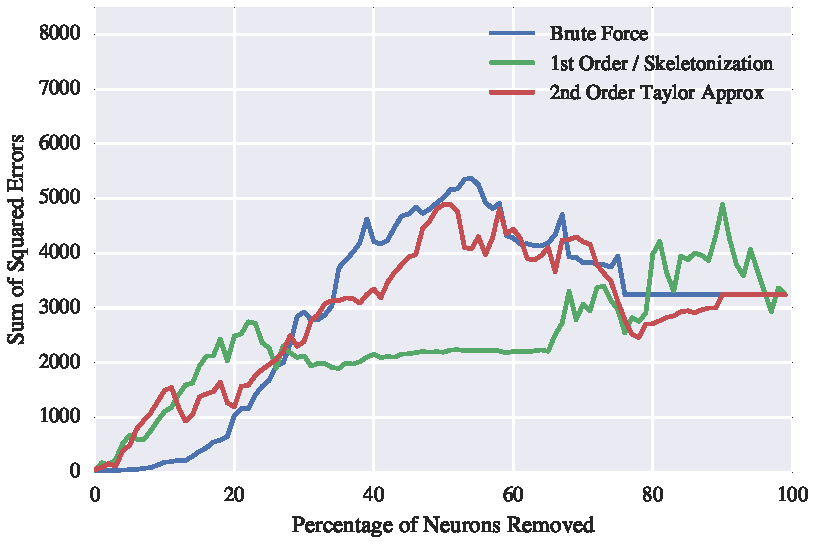
\includegraphics[width=0.49\linewidth]{mnist-deep-single-pass-method.pdf}
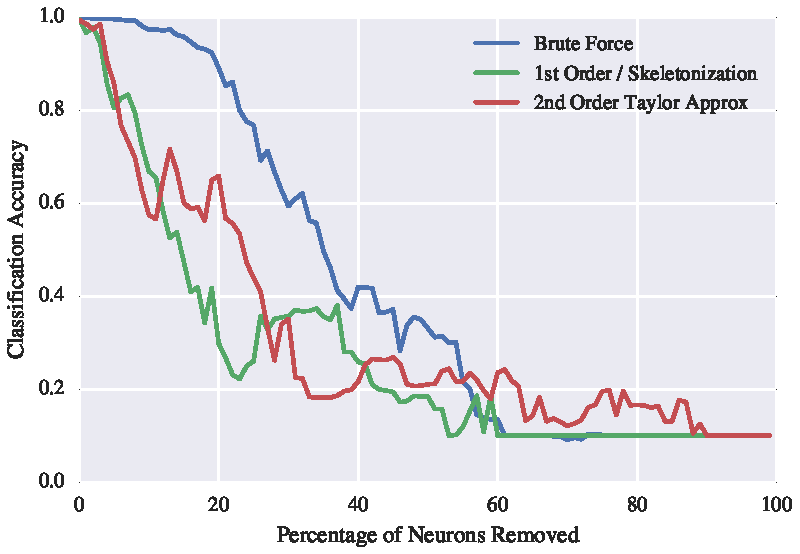
\includegraphics[width=0.49\linewidth]{mnist-deep-single-pass-accuracy.pdf}
\caption{Degradation in squared error (left) and classification accuracy (right) after pruning a 2-layer network using the Single Overall Ranking algorithm; (\textbf{Network:} 2 layers, 50 neurons/layer, 10 outputs, logistic sigmoid activation, starting test accuracy: 1.000)}
\label{fig:mnist-single-ranking-double-layer}
\end{figure}

Figure \ref{fig:mnist-single-ranking-double-layer} shows the pruning results for Algorithm \ref{algo1} on a 2-layer network. The ranking procedure is identical to the one used to generate Figure \ref{fig:mnist-single-ranking-single-layer}. (We again note that this algorithm is intentionally naive and is used for comparison only. Its performance should be expected to be poor.) 

Unsurprisingly, a 2-layer network is harder to prune because a single overall ranking will never capture the interdependencies between neurons in different layers. It makes sense that this is worse than the performance on the 1-layer network, even if this method is already known to be bad, and we'd likely never use it in practice. 

\subsubsection{iterative re-ranking Algorithm}
\begin{figure}[!ht]
\centering
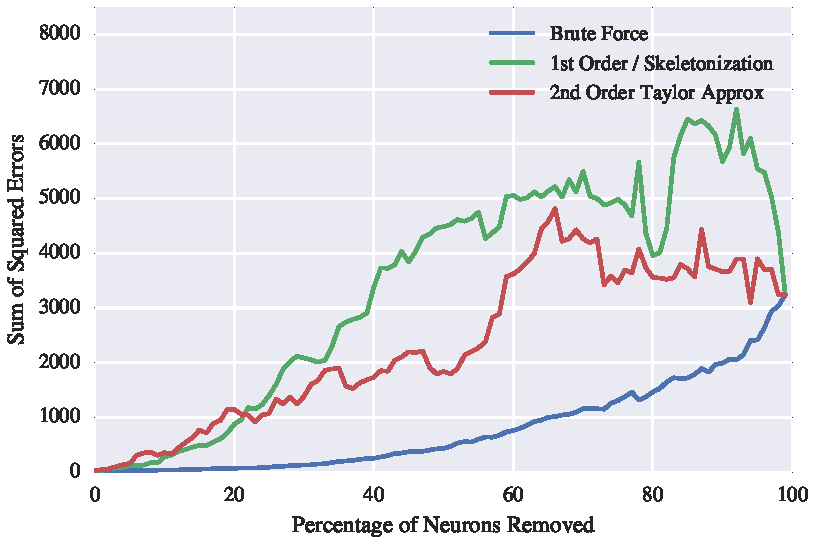
\includegraphics[width=0.49\linewidth]{mnist-deep-iterative-rerank-method.pdf}
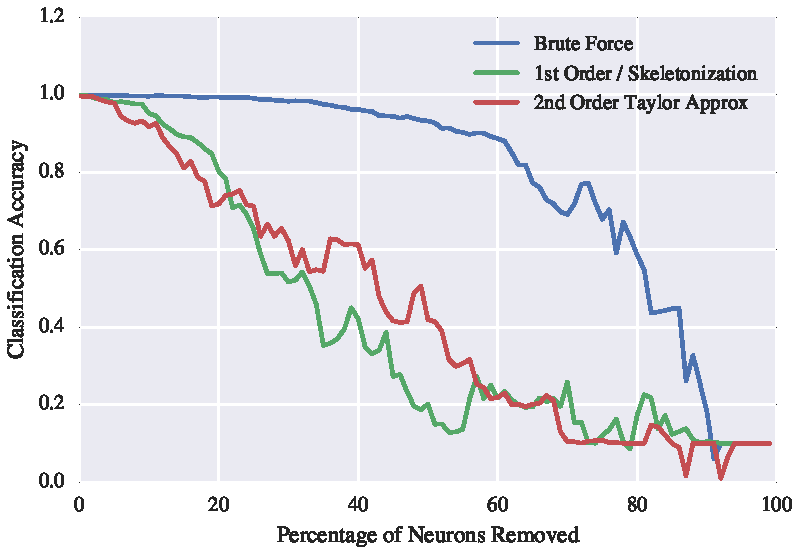
\includegraphics[width=0.49\linewidth]{mnist-deep-iterative-rerank-accuracy.pdf}
\caption{Degradation in squared error (left) and classification accuracy (right) after pruning a 2-layer network using the iterative re-ranking algorithm; (\textbf{Network:} 2 layers, 50 neurons/layer, 10 outputs, logistic sigmoid activation, starting test accuracy: 1.000)}
\label{fig:mnist-re-ranking-double-layer}
\end{figure}

Figure \ref{fig:mnist-re-ranking-double-layer} shows the results from using Algorithm \ref{algo2} on a 2-layer network. We compute the same brute force rankings and Taylor series approximations of error deltas over the remaining active neurons in the network after each pruning decision used to generate Figure \ref{fig:mnist-re-ranking-single-layer}. Again, this is intended to account for the effects of cancelling interactions between neurons. 

It is clear that it becomes harder to remove neurons 1-by-1 with a deeper network (which makes sense because the neurons have more interdependencies in a deeper network), but we see an overall better performance with 2nd order method vs. 1st order, except for the first 20\% of the neurons (but this doesn't seem to make much difference for classification accuracy.) 

Perhaps a more important observation here is that even with a more complex network, it is possible to remove up to 40\% of the neurons with no major loss in performance which is clearly illustrated by the brute force curve. This shows the clear potential of an ideal pruning technique and also shows how inconsistent 1st and 2nd order Taylor Series approximations of the error can be as ranking criteria.

\subsubsection{Visualization of Error Surface \& Pruning Decisions}
As seen in the case of a single layered network, these graphs are a visualization the error surface of the network output with respect to the neurons chosen for removal using each algorithm, represented in intervals of 10 neurons. 

\subsubsection{Visualization of brute force Pruning Decisions}
\begin{figure}[!ht]
\centering
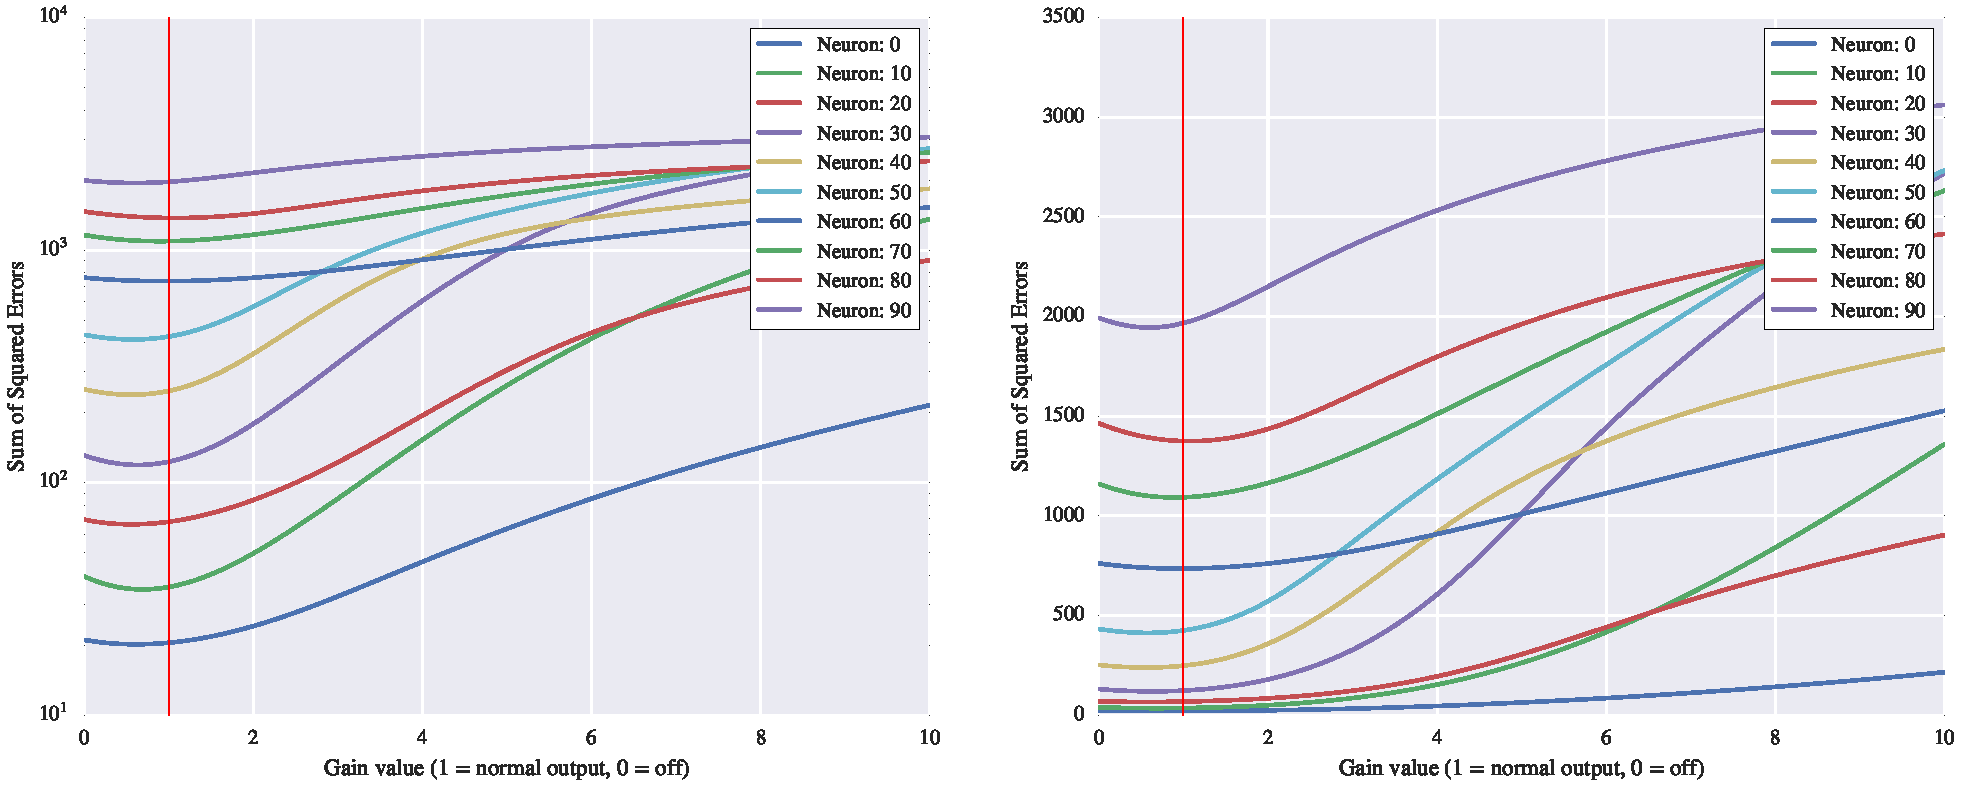
\includegraphics[width=\linewidth]{mnist-deep-gt-gain.pdf}
\caption{Error surface of the network output in log space (left) and real space (right) with respect to each candidate neuron chosen for removal using the brute force criterion; (\textbf{Network:} 2 layers, 50 neurons/layer, 10 outputs, logistic sigmoid activation, starting test accuracy: 1.000)}
\label{fig:mnist-gt-double-layer}
\end{figure}

In Figure \ref{fig:mnist-gt-double-layer}, it is clear why these neurons got chosen, their graphs clearly show little change when neuron is removed, are mostly near the floor, and show convex behaviour of error surface, which argues for the rationalization of using 2nd order methods to estimate difference in error when they are turned off.

\subsubsection{Visualization of 1st Order Approximation Pruning Decisions}
\begin{figure}[!ht]
\centering
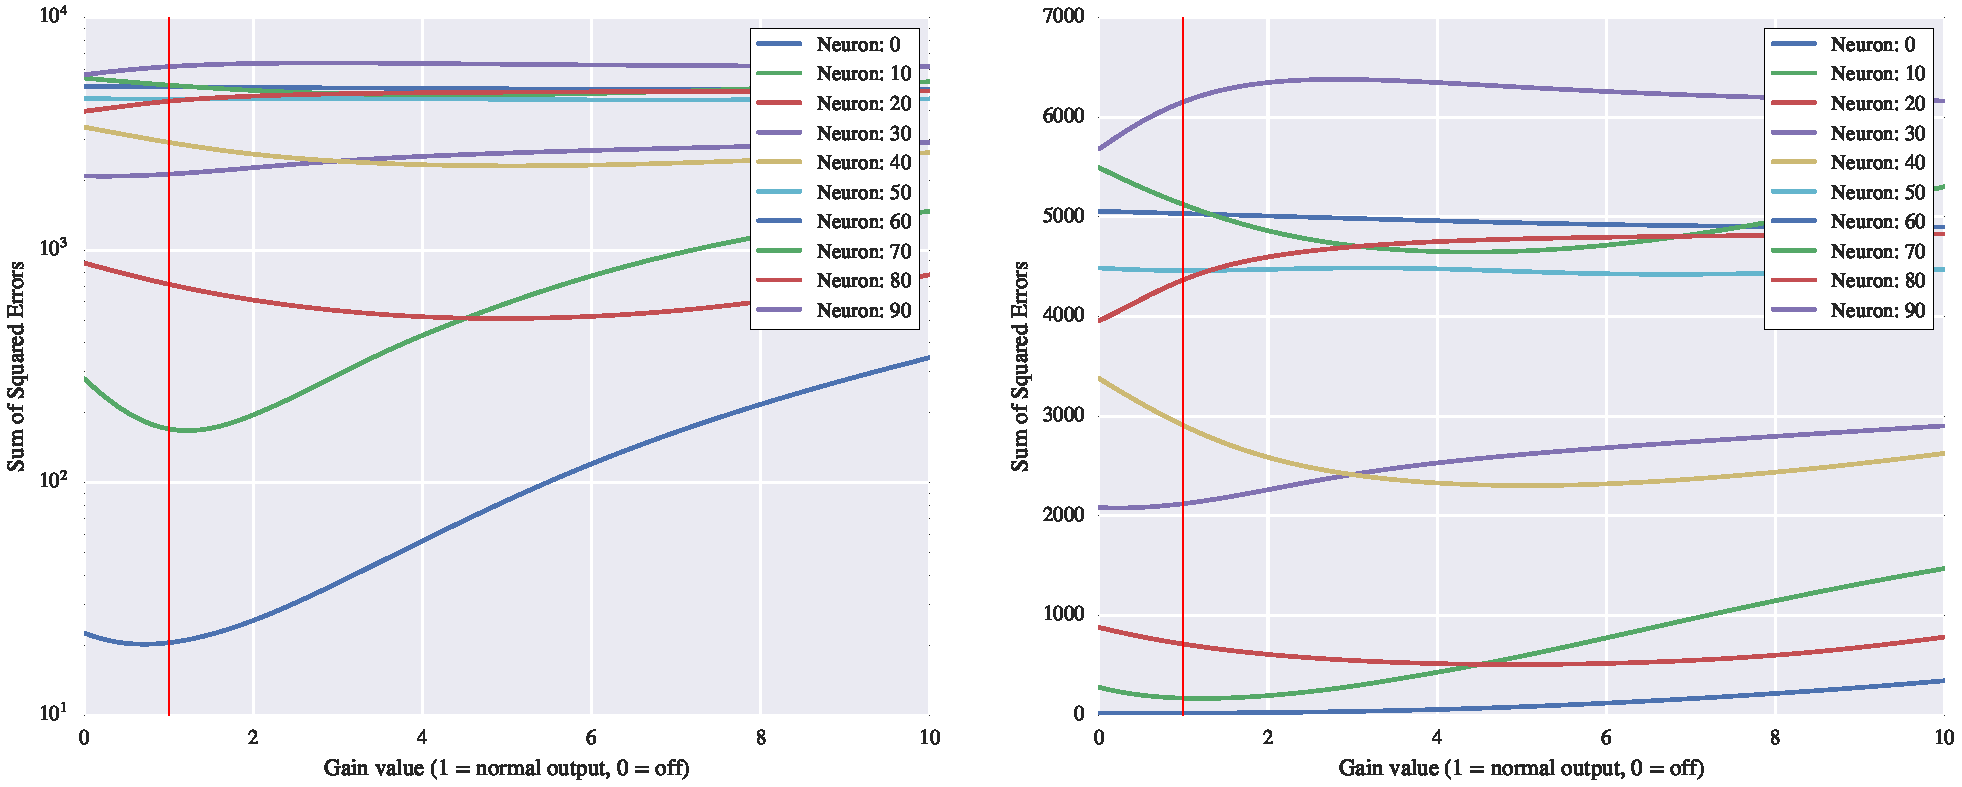
\includegraphics[width=\linewidth]{mnist-deep-g1-gain.pdf}
\caption{Error surface of the network output in log space (left) and real space (right) with respect to each candidate neuron chosen for removal using the 1st order Taylor Series error approximation criterion; (\textbf{Network:} 2 layers, 50 neurons/layer, 10 outputs, logistic sigmoid activation, starting test accuracy: 1.000)}
\label{fig:mnist-g1-double-layer}
\end{figure}

Drawing a flat line at the point of each neurons intersection with the red vertical line (no change in gain) shows that the 1st derivative method is actually accurate for estimation of change in error in these cases, but still ultimately leads to poor decisions. 

\subsubsection{Visualization of 2nd Order Approximation Pruning Decisions}
\begin{figure}[!ht]
\centering
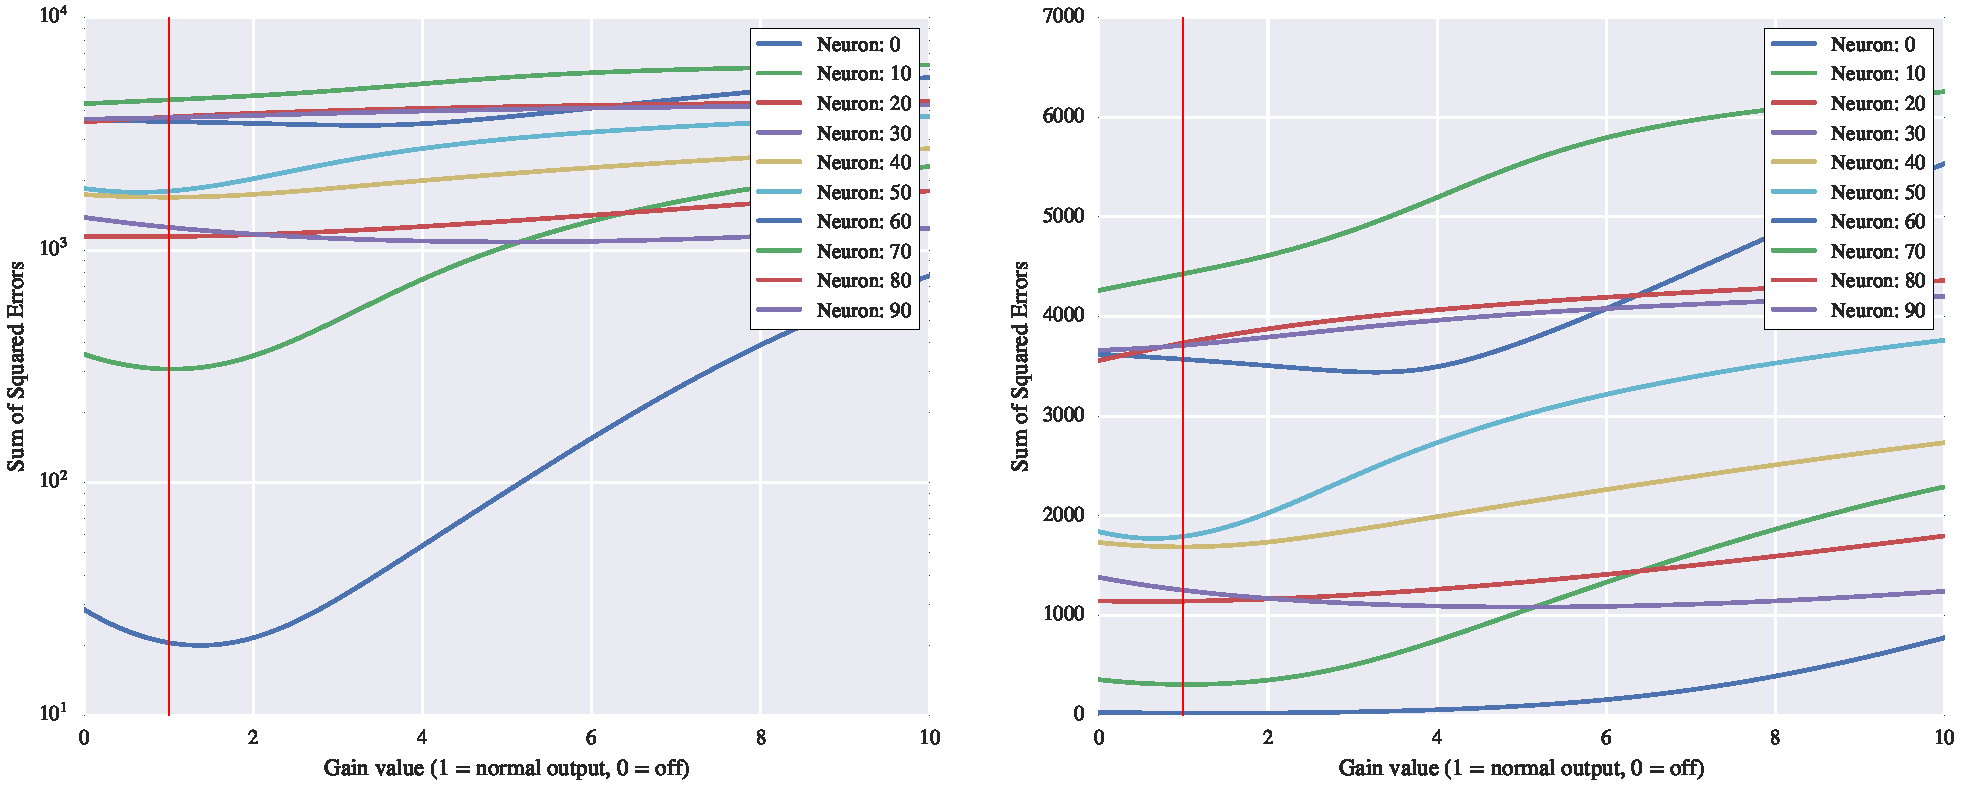
\includegraphics[width=\linewidth]{mnist-deep-g2-gain.pdf}
\caption{Error surface of the network output in log space (left) and real space (right) with respect to each candidate neuron chosen for removal using the 2nd order Taylor Series error approximation criterion; (\textbf{Network:} 2 layers, 50 neurons/layer, 10 outputs, logistic sigmoid activation, starting test accuracy: 1.000)}
\label{fig:mnist-g2-double-layer}
\end{figure}

Clearly these neurons are not overtly poor candidates for removal (error doesn't change much between 1.0 \& zero-crossing left-hand-side), but could be better (as described above in the brute force Criterion discussion).

\subsection{Investigation of Pruning Performance With Imperfect Starting Conditions}

In our experiments thus far we have tacitly assumed that we start with a network which has learned an ``optimal'' representation of the training objective, i.e. it has been trained to the point where we accept its performance on the test set. Here we explore what happens when we prune with a sub-optimal starting network. 

If the assumptions of this paper regarding the nature of neural network learning are correct, we expect that two processes are essentially at work during back-propagation training. First, we expect that the neurons which directly participate in the fundamental learning representation (even if redundantly) work together to reduce error on the training data. Second, we expect that neurons which do not directly participate in the learning representation work to cancel each other's negative influence. Furthermore, we expect that these two groups are essentially distinct, as evinced by the fact that multiple neurons can often be removed as a group with little to no effect on the network output. Some non-trivial portion of the training time, then, is spent doing work which has nothing intrinsically to do with the learning representation and essentially functions as noise cancellation. 

If this is the case, when we attempt to prune a network which has not fully canceled the noisy influence of extraneous or redundant units, we might expect to see the error actually \textit{improve} after removing a few bad apples. This is in fact what we observe, as demonstrated in the following experiments. 

For each experiment in this section we trained with the full MNIST training set (\cite{lecun-mnisthandwrittendigit-2010}), uncompressed and without any data normalization. We trained three different networks to learn to distinguish a single handwritten digit from the rest of the data. The network architectures were each composed of 784 inputs, 1 hidden layer with 100 neurons, and 2 soft-max outputs; one to say yes, and the other to say no. These networks were trained to distinguish the digits 0, 1, and 2, and their respective starting accuracies were a sub-optimal 0.9757, 0.9881, and 0.9513. Finally, we only consider the iterative re-ranking algorithm, as the single overall ranking algorithm is clearly nonviable. 

\subsubsection{MNIST Single Digit Classification: Digit 0}

Figure \ref{fig:mnist-test-single-digit-0} shows the degradation in squared error after removing neurons from a network trained to distinguish the digit 0. What we observe is that the first and second order methods both fail in different ways, though clearly the second order method makes better decisions overall. The first order method explodes spectacularly in the first few iterations. The brute force method, in stark contrast, actually \textit{improves} in the first few iterations, and remains essentially flat until around the 60\% mark, at which point it begins to gradually increase and meet the other curves. 

\begin{figure}[!ht]
\centering
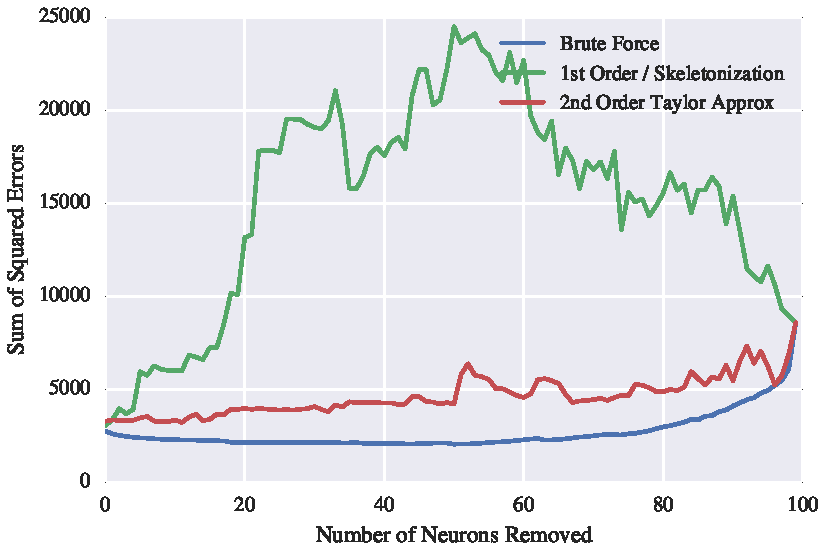
\includegraphics[width=0.5\linewidth]{mnist-test-single-digit-0.pdf}
\caption{Degradation in squared error after pruning a single-layer network trained to do a one-versus-all classification of the digit 0 using the iterative re-ranking algorithm}
\label{fig:mnist-test-single-digit-0}
\end{figure}

The behavior of the brute force method here demonstrates that the network was essentially working to cancel the effect of a few bad neurons when the training convergence criteria were met, i.e. the network was no longer able to make progress on the training set. After removing these neurons during pruning, the output improved. We can investigate this by looking at the error surface with respect to the neurons chosen for removal by each method in turn. Below in Figure \ref{fig:mnist-test-single-digit-0-gt} is the graph of the brute force method. 

\begin{figure}[!ht]
\centering
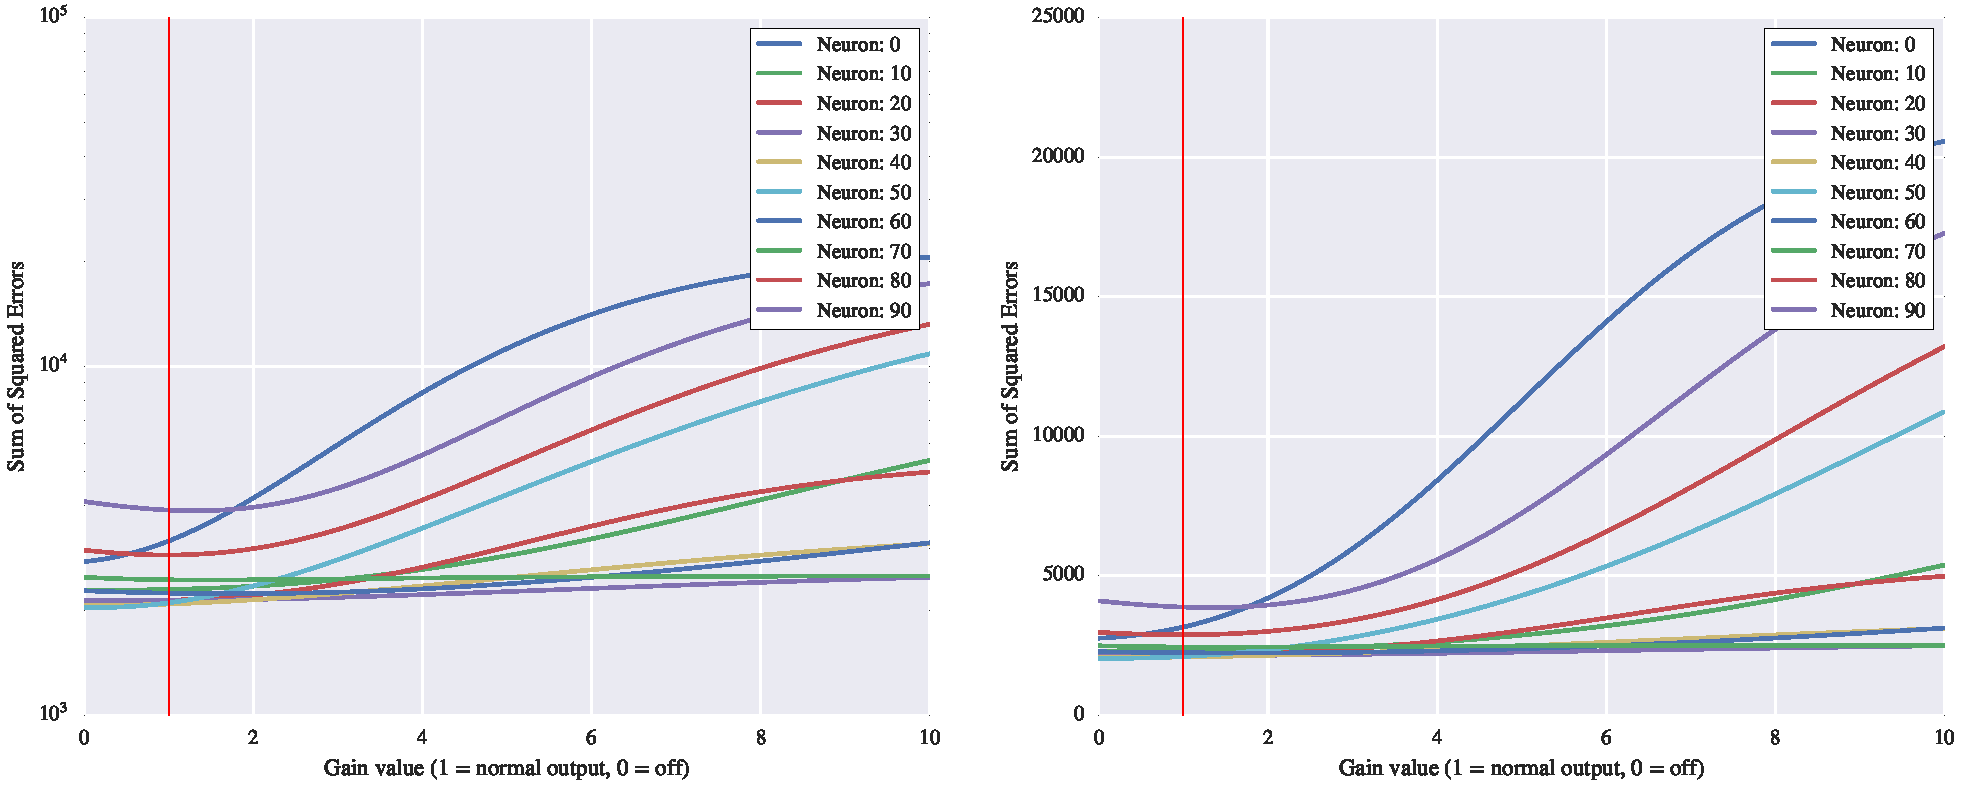
\includegraphics[width=\linewidth]{mnist-test-single-digit-0-gt.pdf}
\caption{Error surface of the network output in log space (left) and real space (right) with respect to each candidate neuron chosen for removal using the brute force iterative re-ranking removal criterion}
\label{fig:mnist-test-single-digit-0-gt}
\end{figure}

Figure \ref{fig:mnist-test-single-digit-0-gt} shows an interesting phenomenon, which we will see in later experiments as well. The high blue curve corresponding to neuron 0 is negatively sloped in the beginning and clearly after removing this neuron, the output will improve. The rest of the curves, in correspondence with the squared error degradation curve above, are mostly flat and tightly layered together, indicating that they are good neurons to remove. 

In Figure \ref{fig:mnist-test-single-digit-0-g1} below, we observe a stark contrast to this. The curves corresponding to neurons 0 and 10 are mostly flat, and fairly lower than the rest, though clearly a mistake was made early on and the rest of the curves are clearly bad choices. In all of these cases however, we see that the curves are easily approximated with a straight line and so the first order method may have been fairly accurate in its predictions, even though it still made poor decisions. 

\begin{figure}[!ht]
\centering
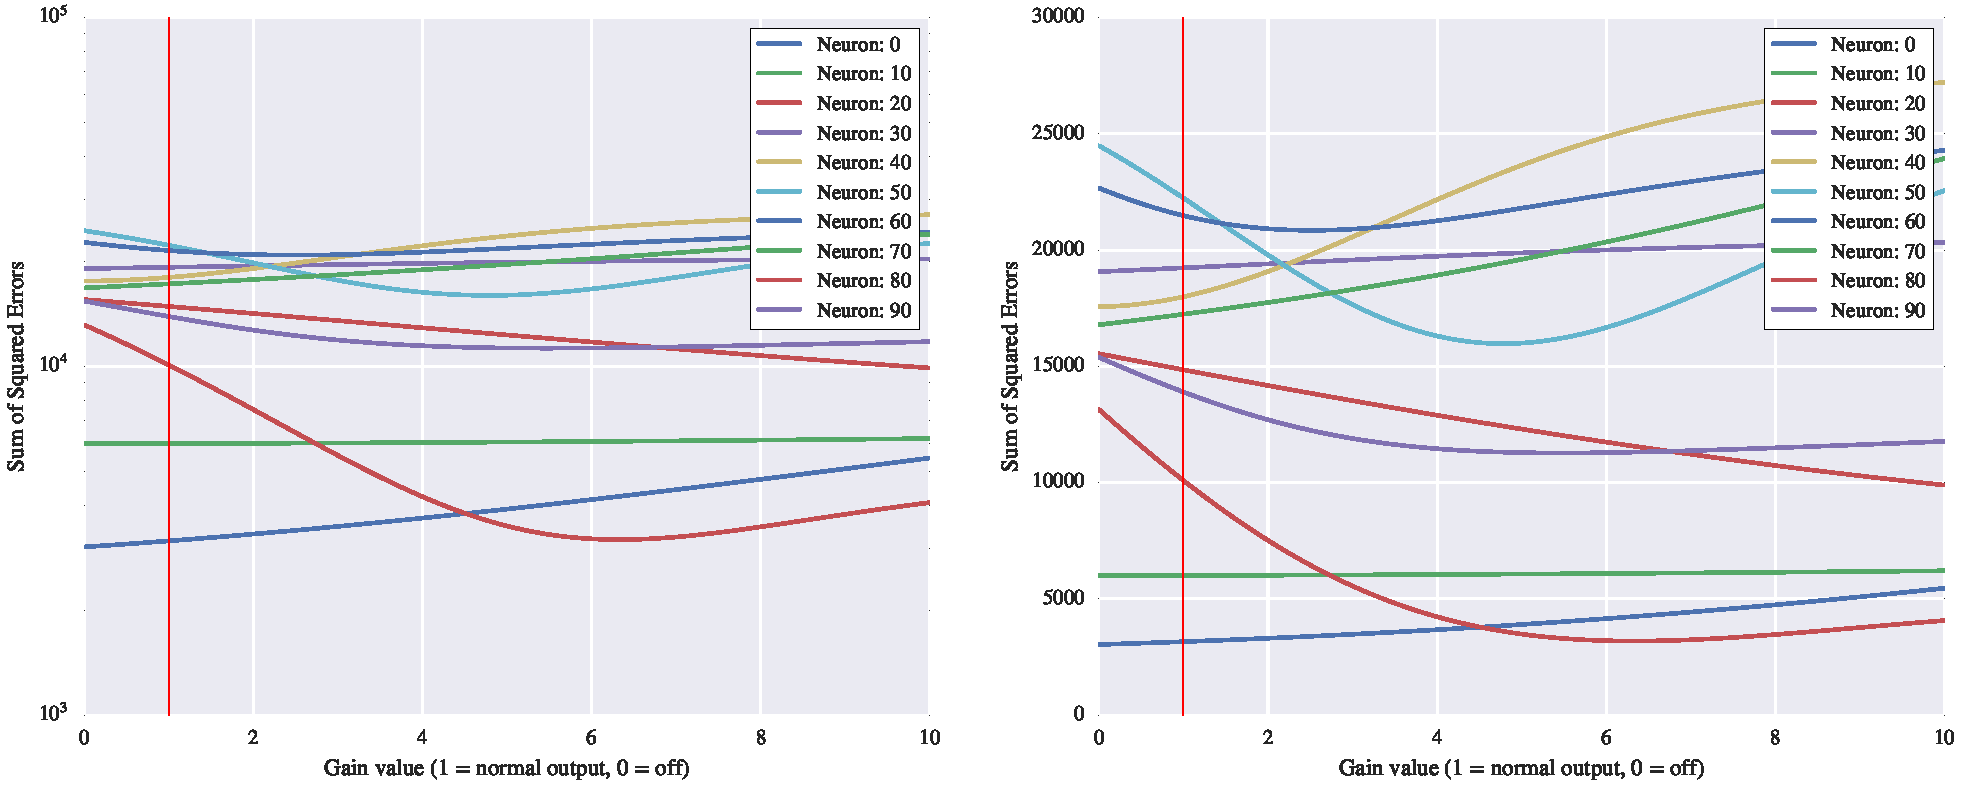
\includegraphics[width=\linewidth]{mnist-test-single-digit-0-g1.pdf}
\caption{Error surface of the network output in log space (left) and real space (right) with respect to each candidate neuron chosen for removal using the first-order iterative re-ranking removal criterion}
\label{fig:mnist-test-single-digit-0-g1}
\end{figure}

Figure \ref{fig:mnist-test-single-digit-0-g1} is an example of how things can go south once a few bad mistakes are made at the outset. Figure \ref{fig:mnist-test-single-digit-0-g2} shows a much better set of choices made by the second order method, though clearly not as good as the brute force method. The log-space plots make it a bit easier to see the difference between the brute force and second order methods in Figures \ref{fig:mnist-test-single-digit-0-gt} and \ref{fig:mnist-test-single-digit-0-g2}, respectively. 

\begin{figure}[!ht]
\centering
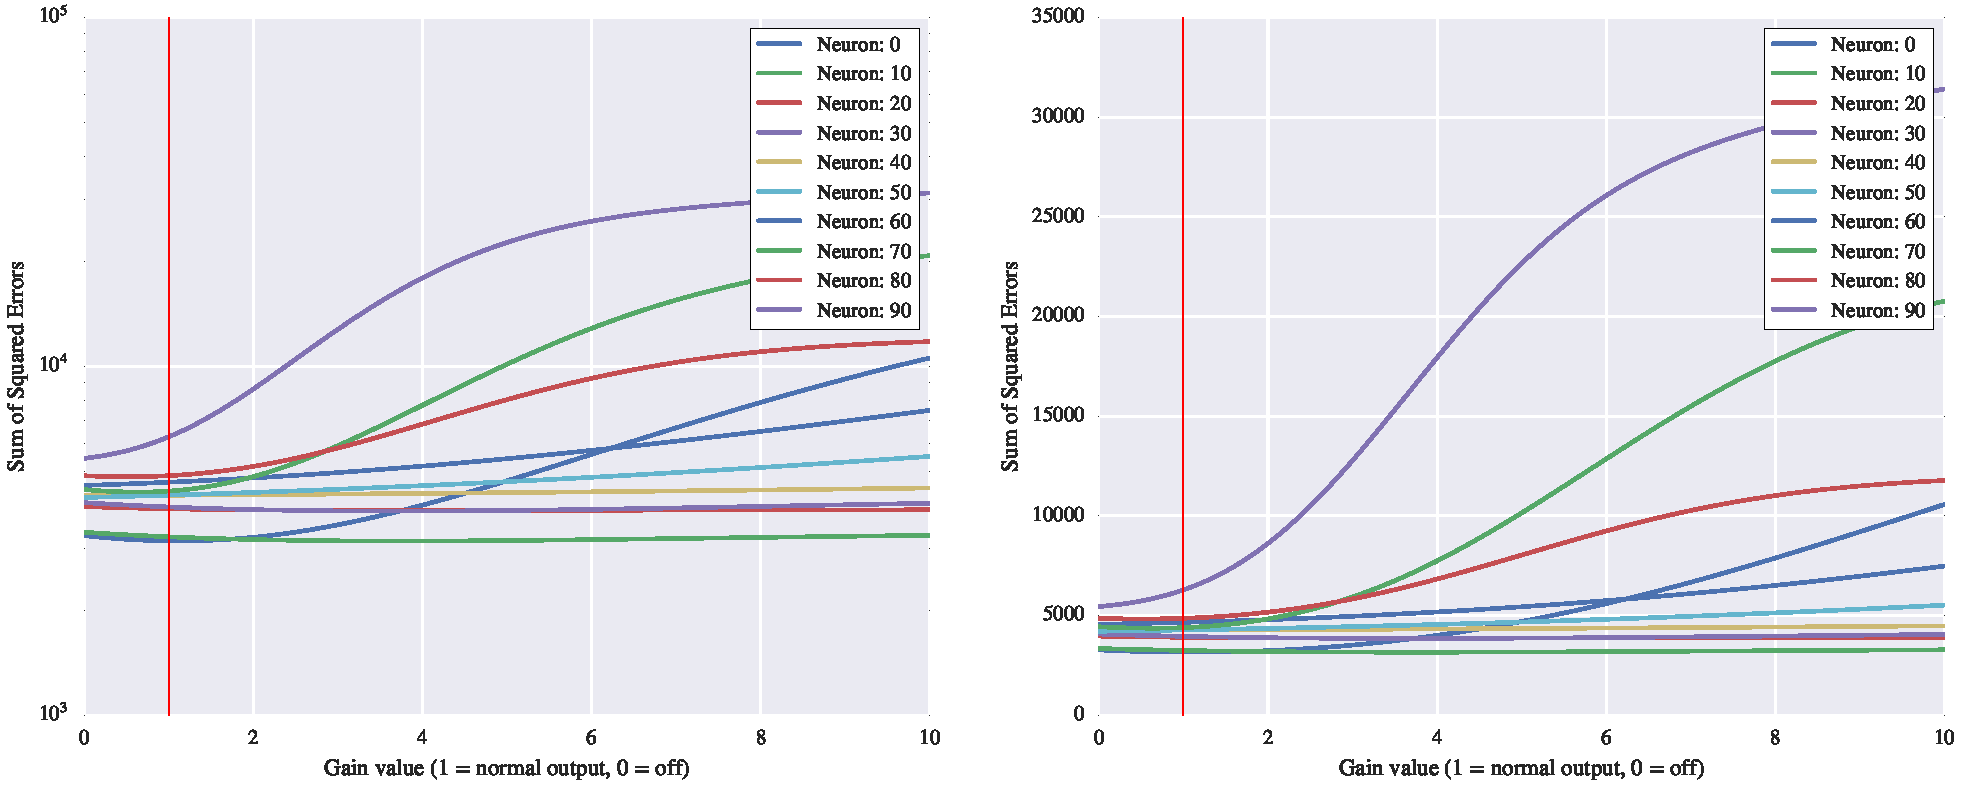
\includegraphics[width=\linewidth]{mnist-test-single-digit-0-g2.pdf}
\caption{Error surface of the network output in log space (left) and real space (right) with respect to each candidate neuron chosen for removal using the second-order iterative re-ranking removal criterion}
\label{fig:mnist-test-single-digit-0-g2}
\end{figure}

\subsubsection{MNIST Single Digit Classification: Digit 1}

Examining Figure \ref{fig:mnist-test-single-digit-1}, we see a much starker example of the previous phenomenon, in which the brute force method continues to \textit{improve} the performance of the network after removing 80\% of the neurons in the network. The first and second order methods fail early and proceed in fits and starts (clearly demonstrating evidence of interrelated groups of noise-canceling neurons), and never fully recover. It should be noted that it would be impossible to see curves like this if neural networks evenly distributed the learning representation evenly or equitably over their hidden units. 

\begin{figure}[!ht]
\centering
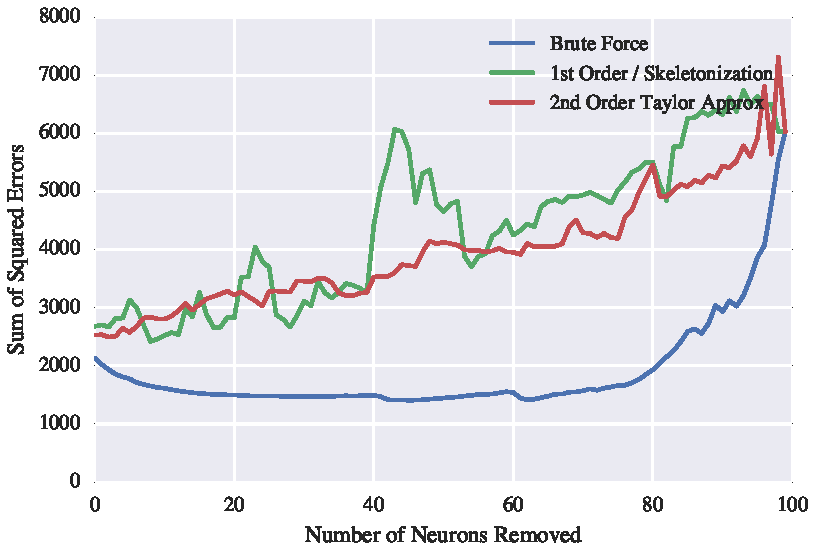
\includegraphics[width=0.5\linewidth]{mnist-test-single-digit-1.pdf}
\caption{Degradation in squared error after pruning a single-layer network trained to do a one-versus-all classification of the digit 1 using the iterative re-ranking algorithm}
\label{fig:mnist-test-single-digit-1}
\end{figure}

One of the most striking things about the blue curve in Figure \ref{fig:mnist-test-single-digit-1} is the fact that the network never drops below its starting error until it crosses the 80\% mark, indicating that only 20\% of the neurons in this network are actually essential to the learning the training objective. In this sense, we can only wonder how much of the training time was spent winnowing the error out of the remaining 80\% of the network. 

\begin{figure}[!ht]
\centering
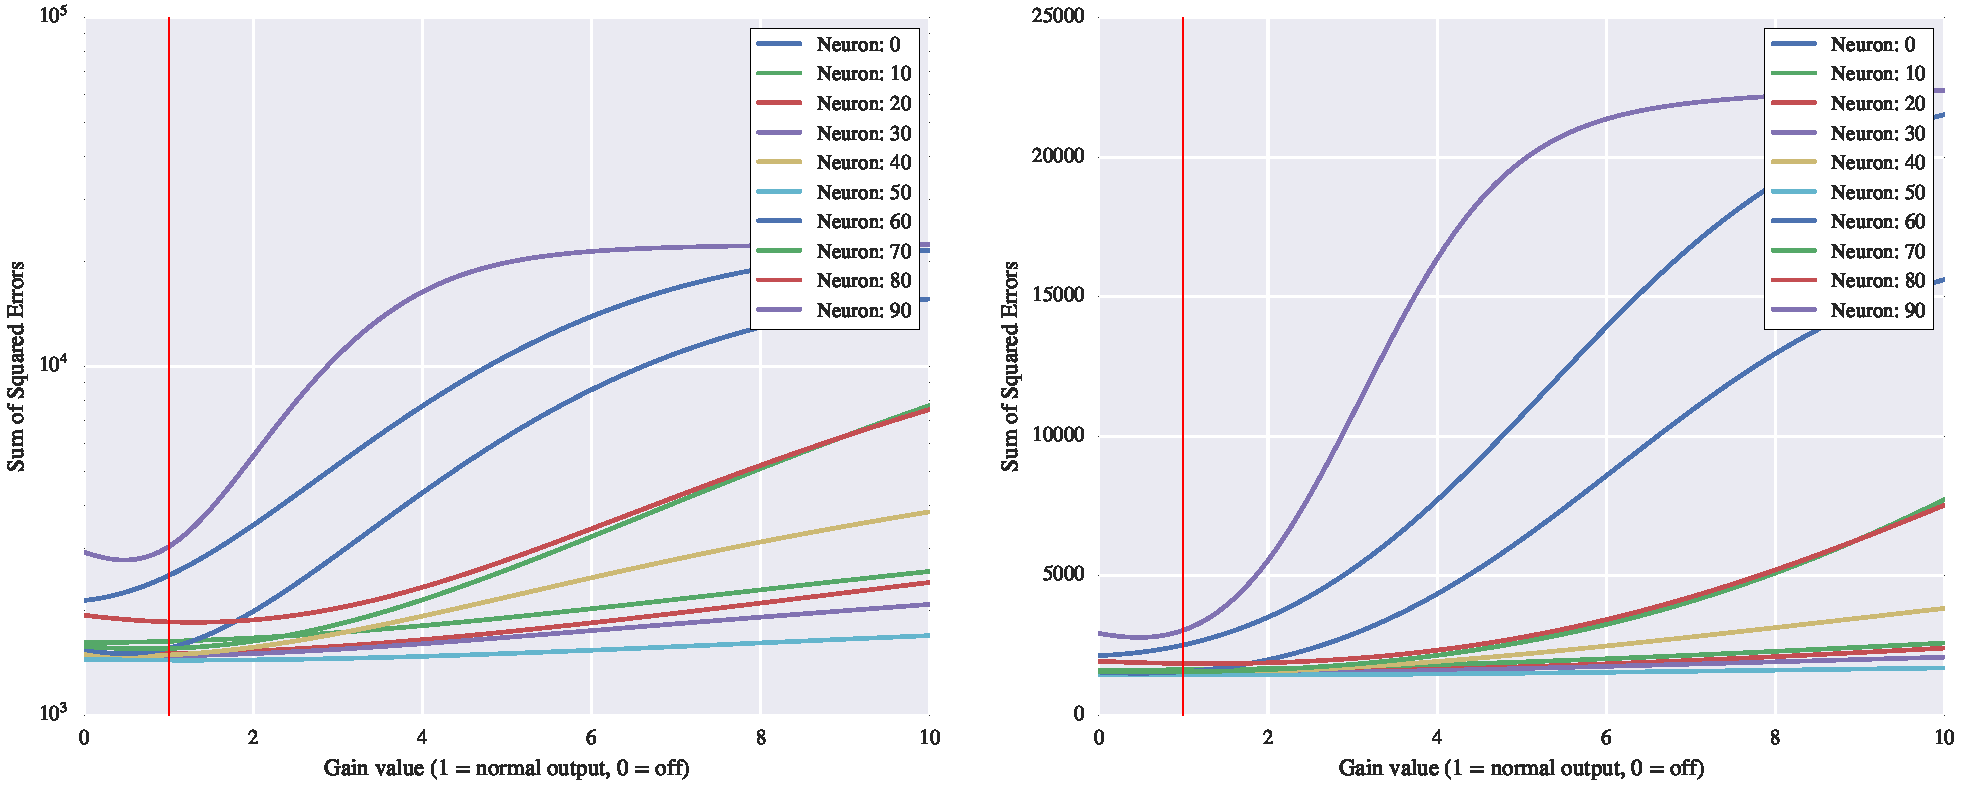
\includegraphics[width=\linewidth]{mnist-test-single-digit-1-gt.pdf}
\caption{Error surface of the network output in log space (left) and real space (right) with respect to each candidate neuron chosen for removal using the brute force iterative re-ranking removal criterion}
\label{fig:mnist-test-single-digit-1-gt}
\end{figure}

In Figures \ref{fig:mnist-test-single-digit-1-gt}, \ref{fig:mnist-test-single-digit-1-g1} and \ref{fig:mnist-test-single-digit-1-g2} we can examine the choices made by the respective methods. The brute force method serves as our example of a near-optimal pruning regimen, and the rest are first and second order approximations of this. Small differences, clearly, can lead to large effects on the network output as shown in Figure \ref{fig:mnist-test-single-digit-1}.

\begin{figure}[!ht]
\centering
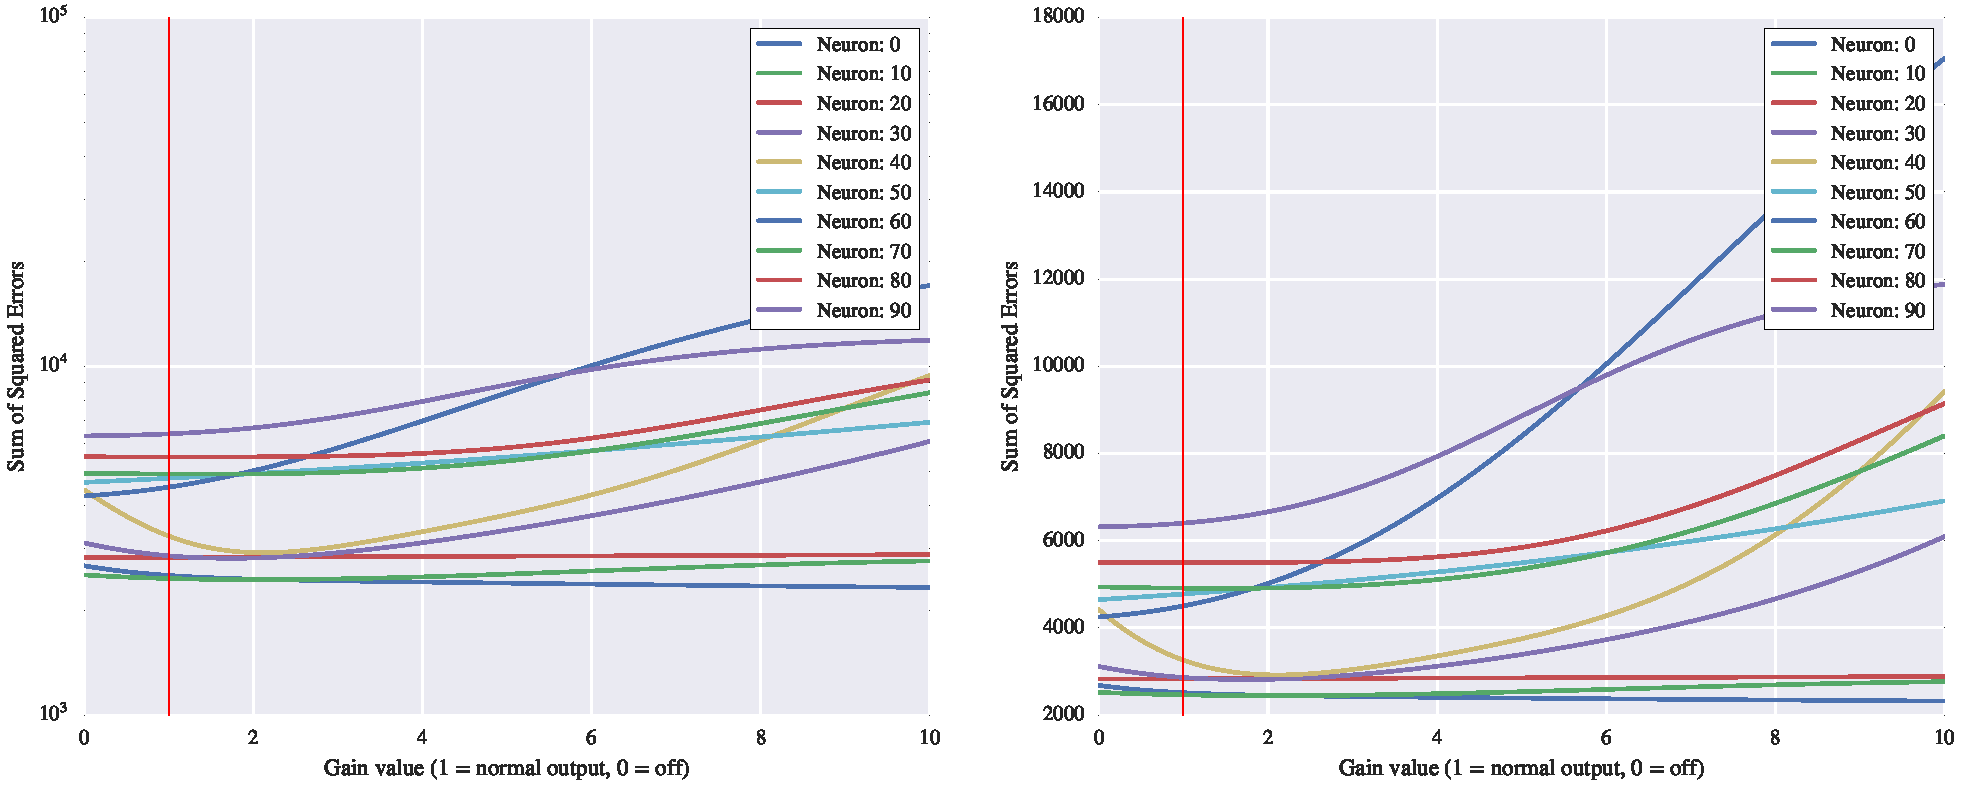
\includegraphics[width=\linewidth]{mnist-test-single-digit-1-g1.pdf}
\caption{Error surface of the network output in log space (left) and real space (right) with respect to each candidate neuron chosen for removal using the first-order iterative re-ranking removal criterion}
\label{fig:mnist-test-single-digit-1-g1}
\end{figure}

\begin{figure}[!ht]
\centering
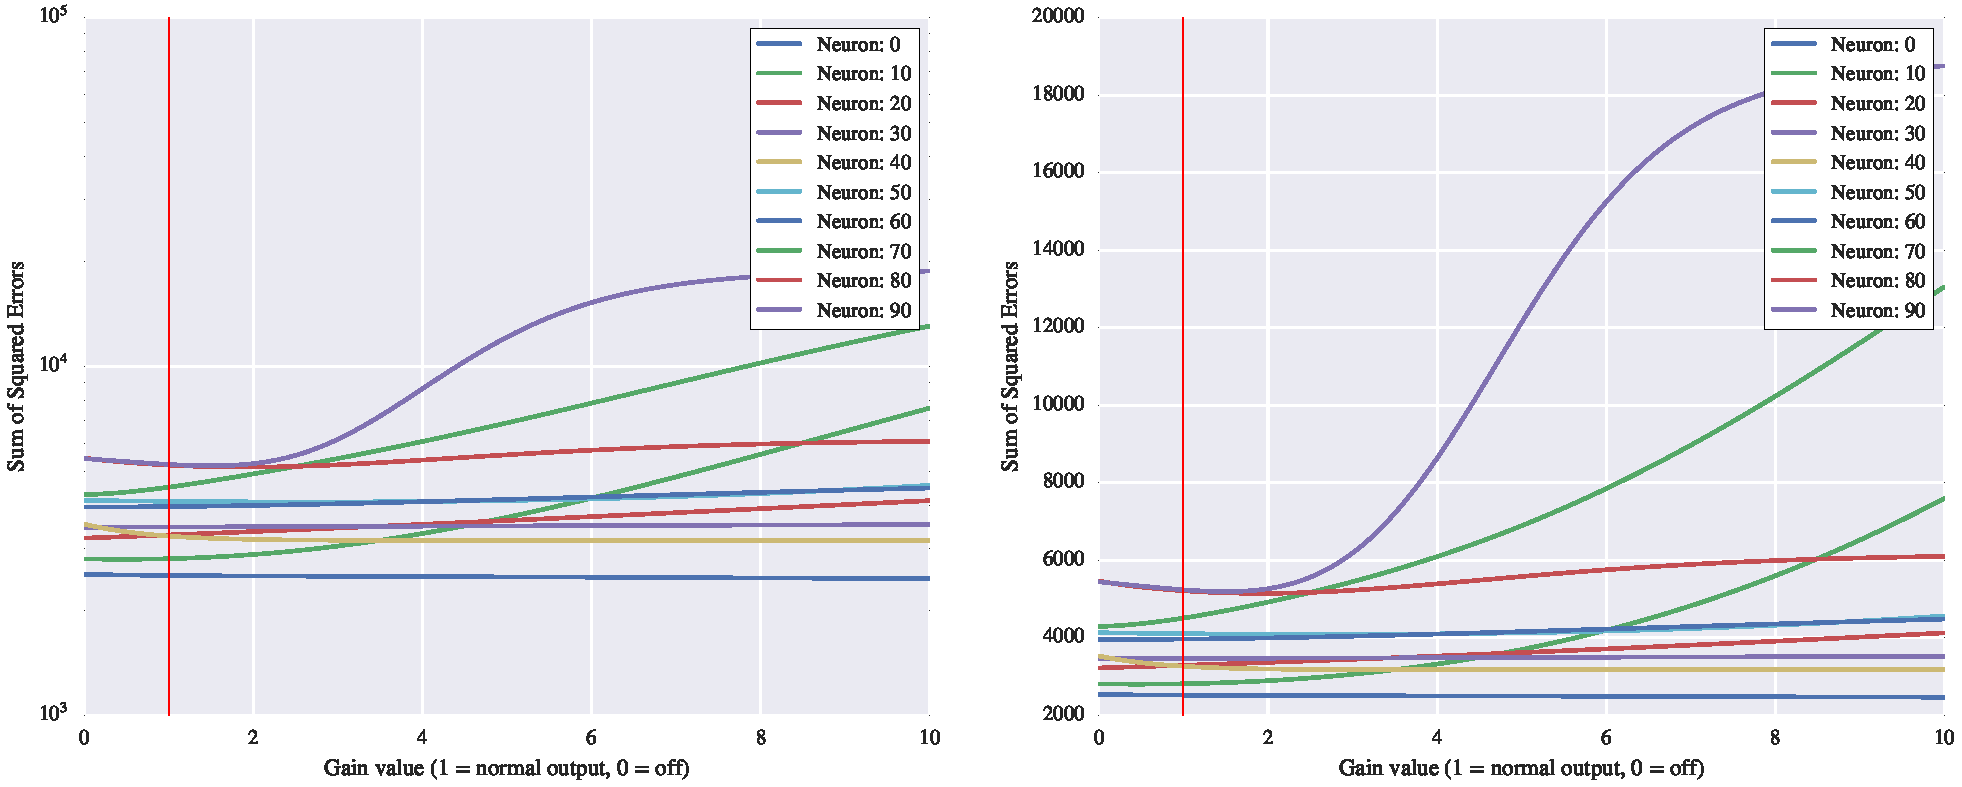
\includegraphics[width=\linewidth]{mnist-test-single-digit-1-g2.pdf}
\caption{Error surface of the network output in log space (left) and real space (right) with respect to each candidate neuron chosen for removal using the second-order iterative re-ranking removal criterion}
\label{fig:mnist-test-single-digit-1-g2}
\end{figure}

\subsubsection{MNIST Single Digit Classification: Digit 2}

Figure \ref{fig:mnist-test-single-digit-2} is an interesting case because it shatters our confidence in the reliability of the second order method to make good pruning decisions, and further demonstrates the phenomenon of how much the error can improve if the right neurons are removed after training gets stuck. In this case, though still a poor performance overall, the first order method vastly outperforms the second order method. 

Figure \ref{fig:mnist-test-single-digit-2-gt} shows us a clear example of the first element to remove having a negative error slope, and improving the output as a result. The rest of the pruning decisions are reasonable. Comparing with the blue curve in Figure \ref{fig:mnist-test-single-digit-2}, we see the correspondence between the first pruning decision improving the output, and the remaining pruning decisions keeping the output fairly flat. Clearly, however, there isn't much room to get worse given our starting point with a sub-optimal network, and we see that the ending sum of squared errors is not much higher than the starting point. At the same time, we can still see the contrast in performance if we make optimal pruning decisions, and most of the neurons in this network were clearly doing nothing. 

\begin{figure}[!ht]
\centering
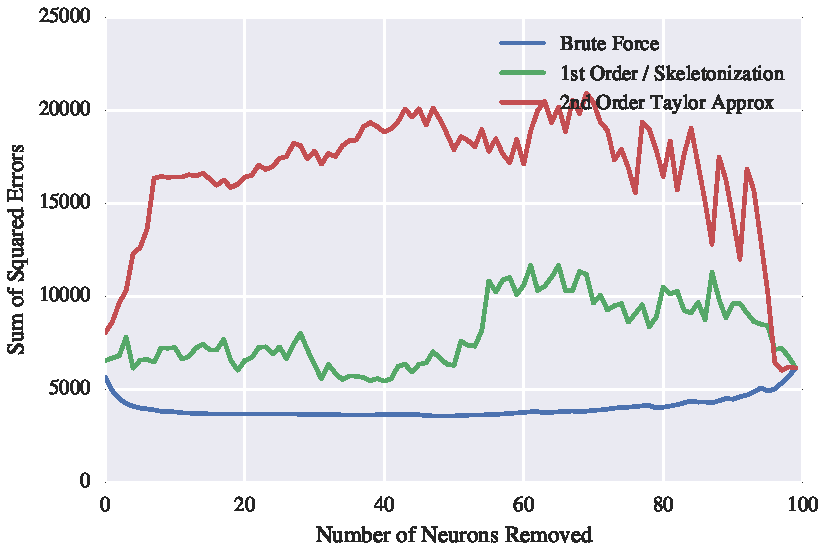
\includegraphics[width=0.5\linewidth]{mnist-test-single-digit-2.pdf}
\caption{Degradation in squared error after pruning a single-layer network trained to do a one-versus-all classification of the digit 2 using the iterative re-ranking algorithm}
\label{fig:mnist-test-single-digit-2}
\end{figure}

\begin{figure}[!ht]
\centering
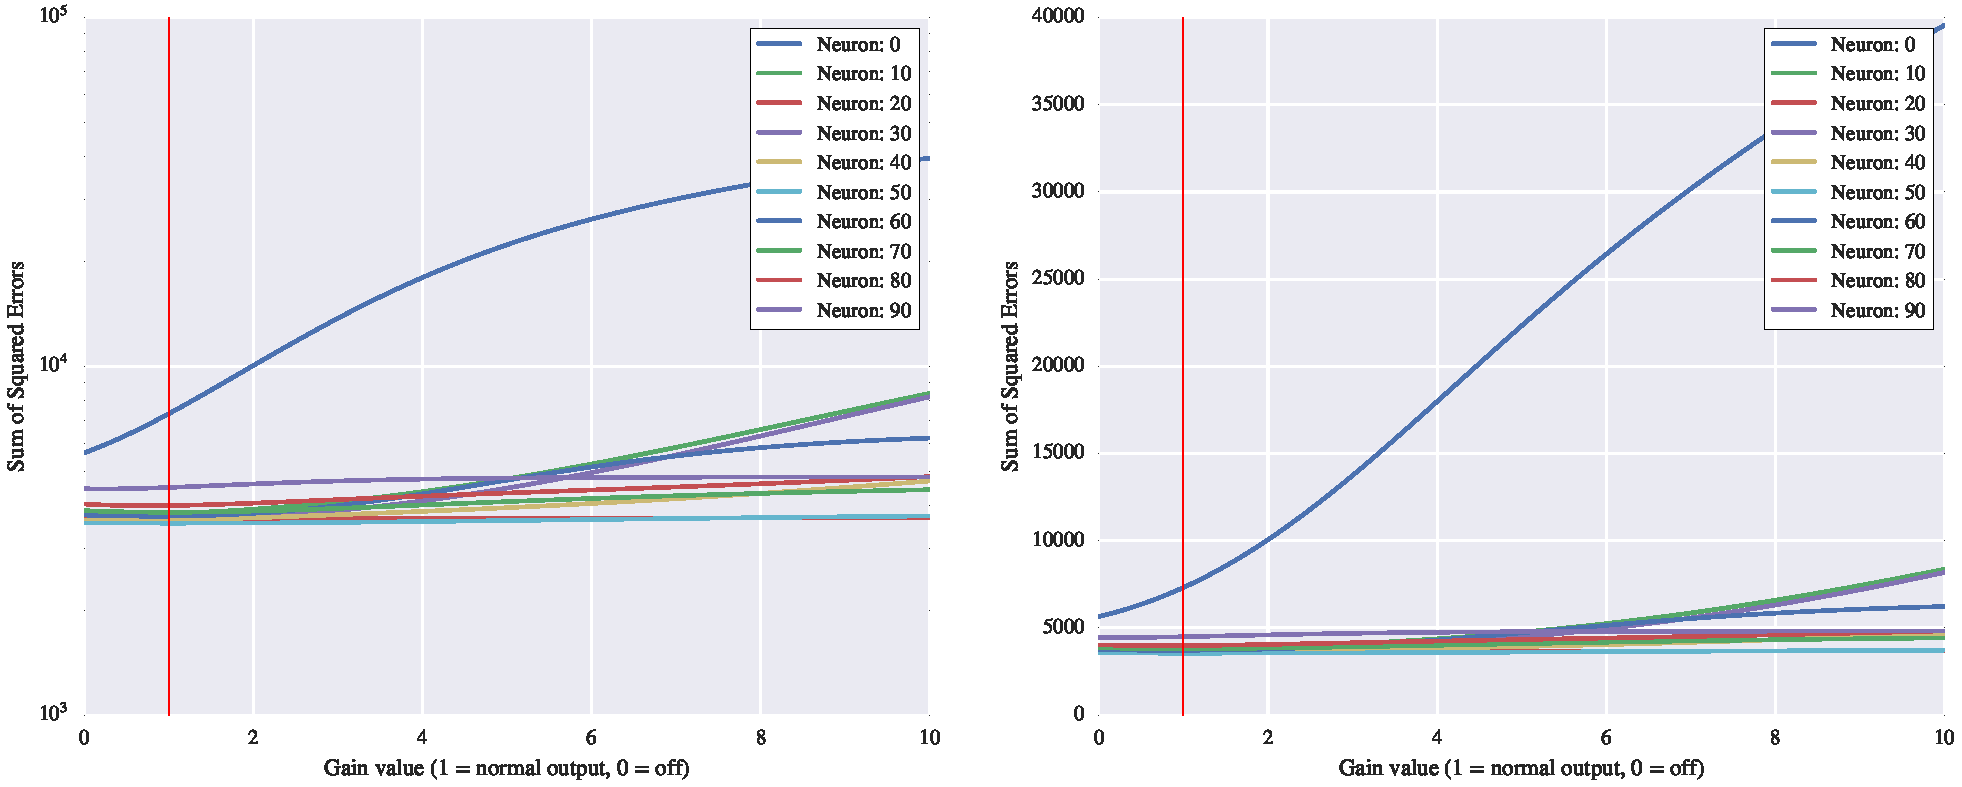
\includegraphics[width=\linewidth]{mnist-test-single-digit-2-gt.pdf}
\caption{Error surface of the network output in log space (left) and real space (right) with respect to each candidate neuron chosen for removal using the brute force iterative re-ranking removal criterion}
\label{fig:mnist-test-single-digit-2-gt}
\end{figure}

In Figure \ref{fig:mnist-test-single-digit-2-g1}, we see a mixed bag in which the decisions are clearly sub-optimal, though much better than Figure \ref{fig:mnist-test-single-digit-2-g2}, in which we can observe how a bad first decision essentially ruined the network for good. The jagged edges of the red curve in Figure \ref{fig:mnist-test-single-digit-2} correspond with the positive and negative slopes of the cluster of bad pruning decisions in \ref{fig:mnist-test-single-digit-2-g2}. Once again, these are not necessarily bad decisions, but the starting point is already bad and this cannot be recovered without re-training the network. 

\begin{figure}[!ht]
\centering
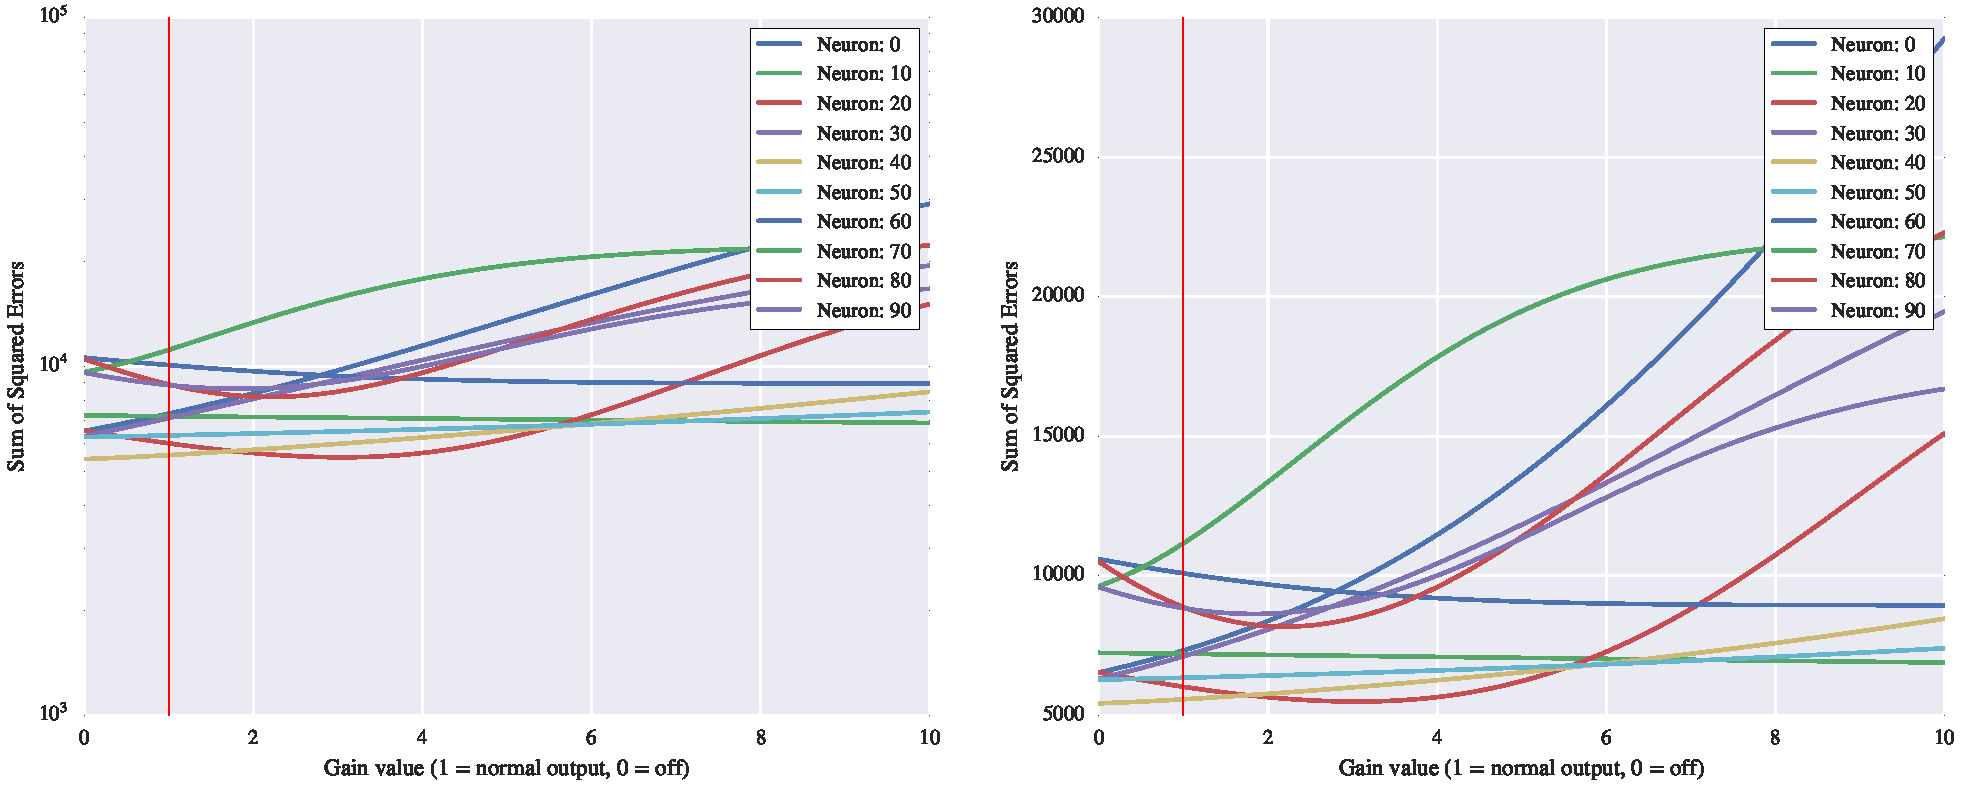
\includegraphics[width=\linewidth]{mnist-test-single-digit-2-g1.pdf}
\caption{Error surface of the network output in log space (left) and real space (right) with respect to each candidate neuron chosen for removal using the first-order iterative re-ranking removal criterion}
\label{fig:mnist-test-single-digit-2-g1}
\end{figure}

\begin{figure}[!ht]
\centering
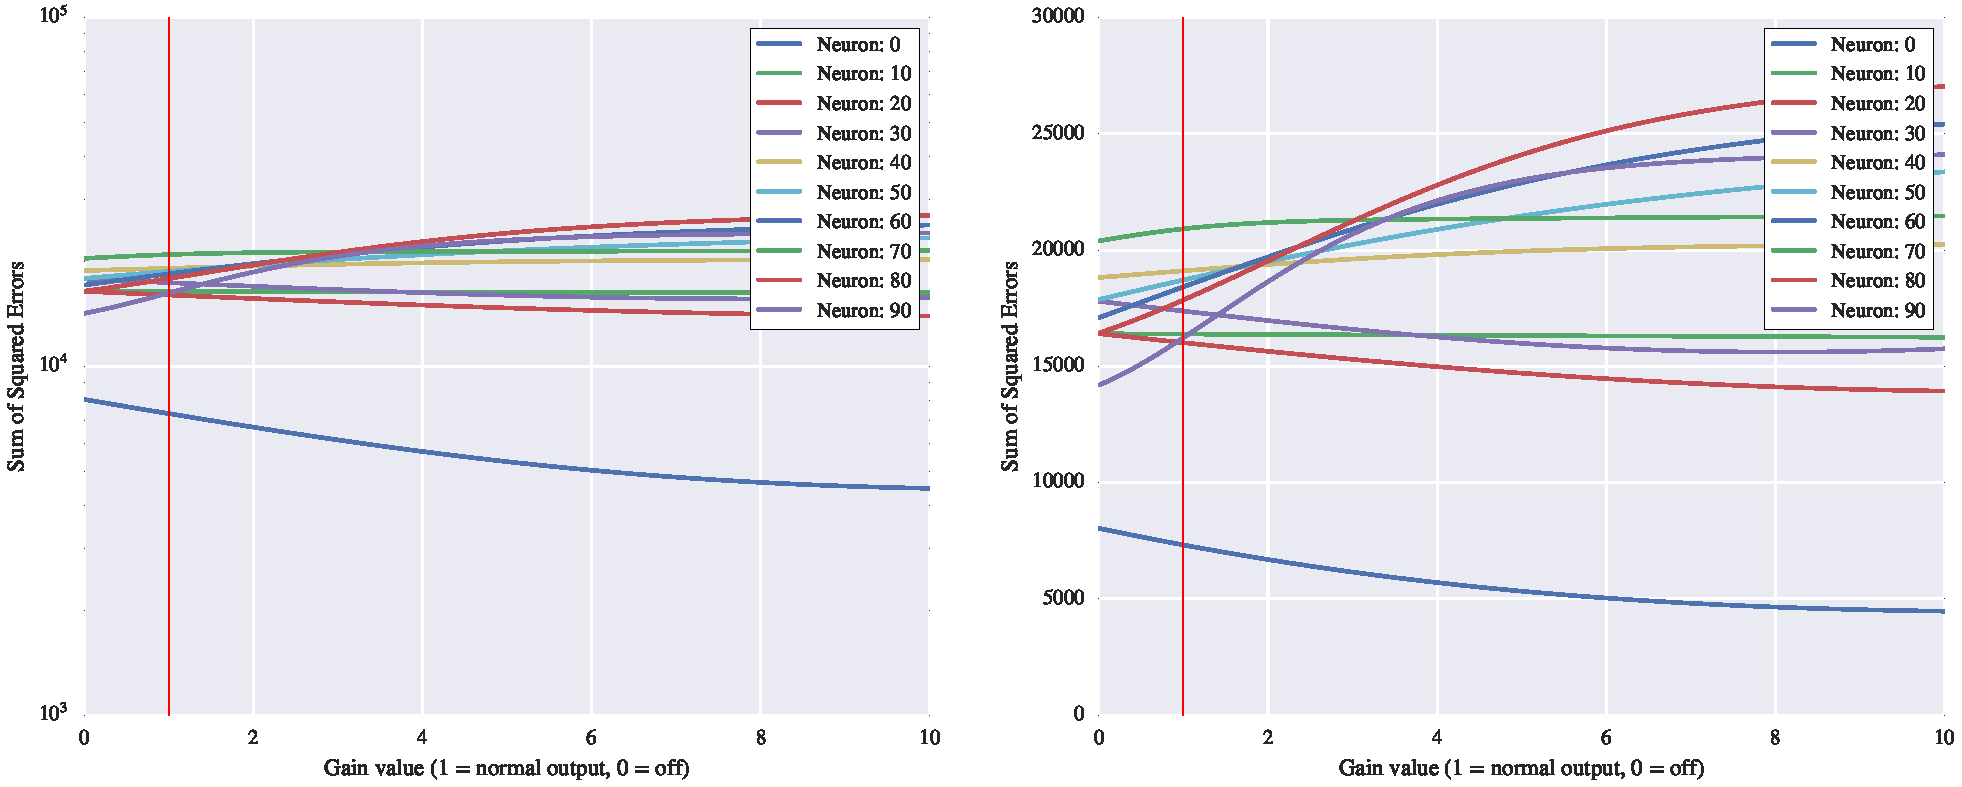
\includegraphics[width=\linewidth]{mnist-test-single-digit-2-g2.pdf}
\caption{Error surface of the network output in log space (left) and real space (right) with respect to each candidate neuron chosen for removal using the second-order iterative re-ranking removal criterion}
\label{fig:mnist-test-single-digit-2-g2}
\end{figure}

\subsubsection{Aside: Implications of This Experiment}

From the three examples above, we see that in each case, starting from a sub-optimal network, a brute force removal technique consistently improves performance for the first few pruning iterations, and the sum of squared errors does not degrade beyond the starting point until around 60-80\% of the neurons have been removed. This is only possible if we have an essentially strict dichotomy between the roles of different neurons during training. If the network needs only 20-40\% of the neurons it began with, the training process is essentially dominated by the task of canceling the residual noise of redundant neurons. Furthermore, the network can get stuck in training with redundant units and distort the final output. This is strong evidence of our thesis that the learning representation is neither equitably nor evenly distributed and that most of the neurons which do not directly participate in the learning representation can be removed without any retraining. 

\subsection{Experiments on Toy Datasets}

As can be seen from the experiments on MNIST, even though the 2nd-order approximation criterion is consistently better than 1st-order, its performance is not nearly as good as brute force based ranking, especially beyond the first layer. What is interesting to note is that from some other experiments conducted on toy datasets (predicting whether a given point would lie inside a given shape on the Cartesian plane), the performance of the 2nd-order method was found to be exceptionally good and produced results very close to the brute force method. The 1st-order method, as expected, performed poorly here as well. Some of these results are illustrated in Figure \ref{fig:diamond}. 

\begin{figure}[!ht]
\centering
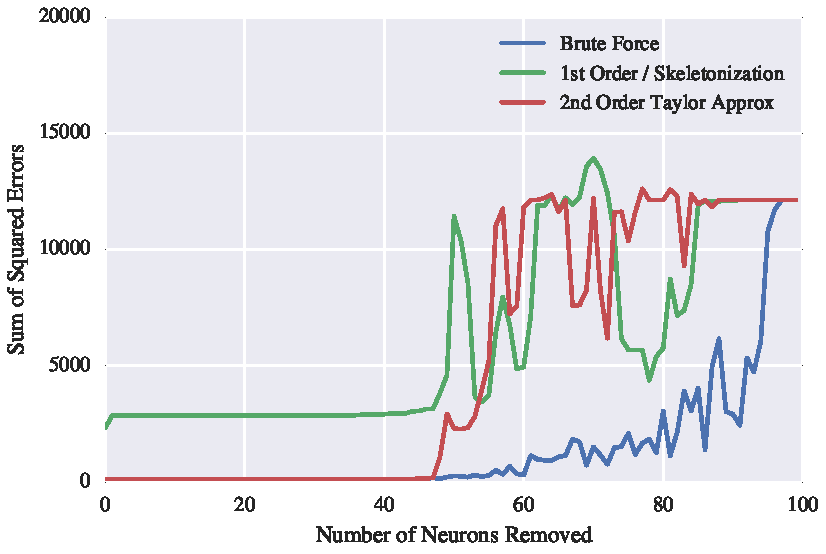
\includegraphics[width=0.49\linewidth]{diamond-iterative-rerank-method.pdf}
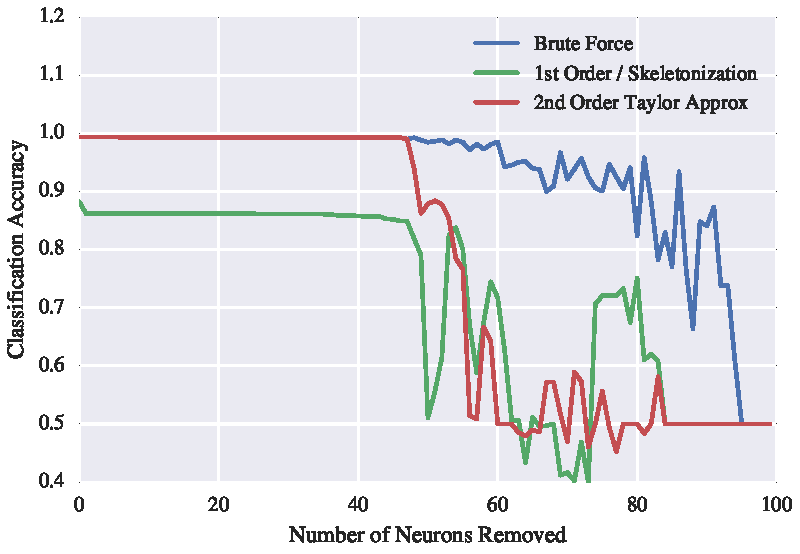
\includegraphics[width=0.49\linewidth]{diamond-iterative-rerank-accuracy.pdf}
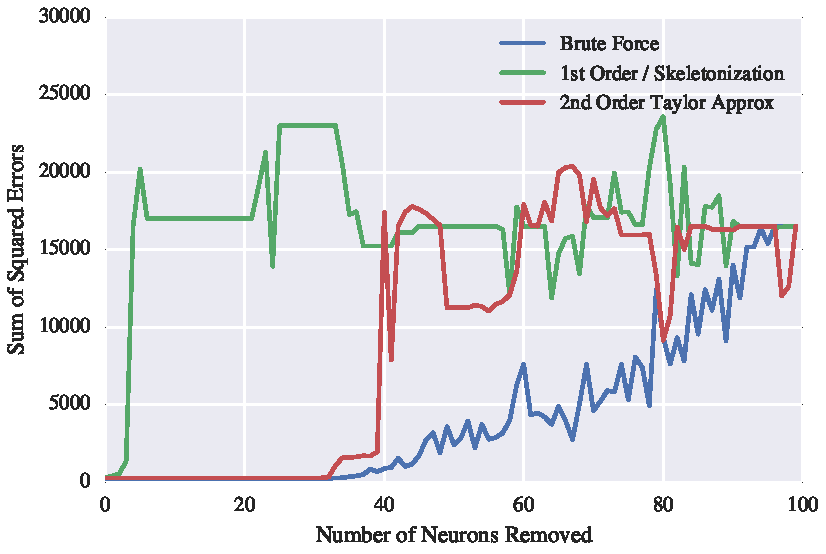
\includegraphics[width=0.49\linewidth]{rshape-iterative-rerank-method.pdf}
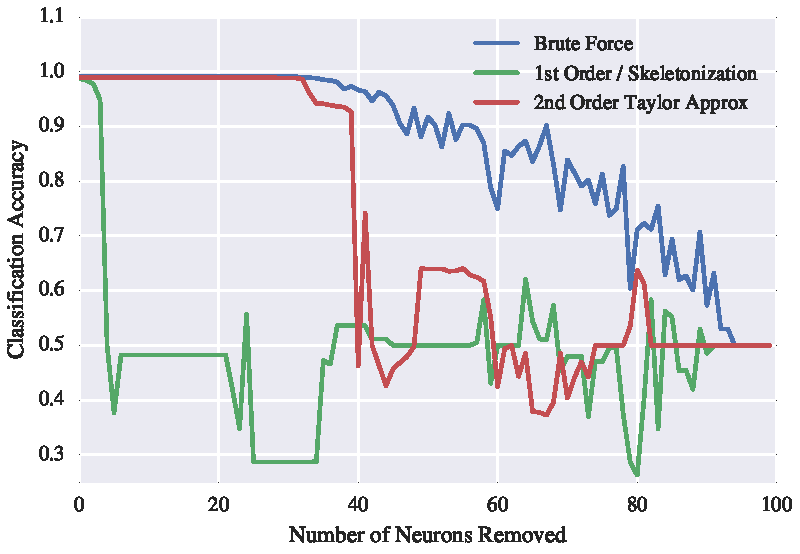
\includegraphics[width=0.49\linewidth]{rshape-iterative-rerank-accuracy.pdf}
\caption{Degradation in squared error (left) and classification accuracy (right) after pruning a 2-layer network using the iterative re-ranking algorithm on a toy ``diamond'' shape dataset (top) and a toy ``random shape'' dataset (below); (\textbf{Network:} 2 layers, 50 neurons/layer, 10 outputs, logistic sigmoid activation, starting test accuracy: 0.992(diamond); 0.986(random shape)}
\label{fig:diamond}
\end{figure}

%This huge variation in results from MNIST might be attributed to the fact that these toy datasets had only 2 output classes (as opposed to 10 classes in MNIST), but it certainly warrants further investigation.